\chapter{Diseño y análisis de datos}
\label{cha:analisis}

Este Capítulo abordará la fase del \gls{tfm} que se centra en el análisis, diseño y procesado de las fuentes de datos para lograr el objetivo principal de generar un dataset final que suponga la base del entrenamiento y el desarrollo de los modelos de \gls{ml} que se plantearán en el Capítulo \ref{cha:desarrollo}. Se abrirá el Capítulo con una Sección enfocada al estudio de la disponibilidad de fuentes de datos de implementaciones reales de \gls{sg}s. Por ello, será imprescindible llevar a cabo una investigación exhaustiva y un posterior análisis de su utilidad en referencia a las necesidades que presenta este \gls{tfm} (ver Sección \ref{sec:sustdata}).

\vspace{3mm}

Por consiguiente, se añadirá una Sección en referencia al estudio de la generación energética (ver Sección \ref{sec:simuprod}). Esta vendrá justificada por la necesidad de realizar un análisis sobre algunas herramientas de simulación existentes que proporcionan datos de potencia. Este proceso posibilitará obtener información adicional sobre los recursos solares y las condiciones climáticas de una ubicación determinada. Una vez expuestas y seleccionadas las fuentes de datos que servirán como base para el desarrollo de este \gls{tfm}, se añadirá una Sección dedicada a la definición detallada de las acciones que serán necesarias para llevar a cabo un procesamiento exhaustivo de toda la información recopilada (ver Sección~\ref{sec:preprocesado}). 

\vspace{3mm}

Después, siguiendo las especificaciones expuestas anteriormente en la Sección \ref{sec:brite}, se plantearán una serie de escenarios mediante la generación de múltiples topologías con la herramienta BRITE (ver Sección \ref{sec:ejebrite}). Los resultados que se obtengan a partir de ella se constituirán como la base sobre la que se realizarán las simulaciones en el algoritmo \gls{den2ne}. En esta Sección (ver Sección \ref{sec:cambiosden2ne}) será preciso detallar las modificaciones y ajustes a implementar en el algoritmo. Esto permitirá extraer a la salida del mismo el conjunto de datos final sobre el que se entrenarán los modelos de \gls{ml} y \gls{dl}.

\vspace{3mm}

% %%%%%%%%%%%%%%%%%%%%%%%%%%%%%%%%%%%%%%%%%%%%%%%%%%%%%%%%%%%%%%%%%%%%%%%%%%%%%%%%%%%%%%%%%%%%%%%%%
<<<<<<< HEAD
%%%%%%%%%%%%%%%%%%%%%%%%%%%%%%%%%%%%%%%%%%%%%%%%%%%%%%%%%%%%%%%%%%
\section{Análisis de fuentes de datos}
\label{sec:sustdata}

%aqui explicar los datasets que se han visto
%enfocarlo mas a todos lo datasets o a sustdata?
%aqui habria que explicar tambien la creacion de los datos de produccion


\cite{sustdata}





%hacer intro en relacion con el apartado de big data

%%para intro -->

%cite stab

%There are two main types of renewable energy data: geospatial and
% temporal data. Geospatial data is concerned with the locations, while
% temporal data is concerned with data time characteristics. For renewable energy, Geospatial data may include the location of transmission
% infrastructure, cities, factories, hospitals, schools, roads, etc. (Shekhar
% et al., 2012); this data is based mainly on Geographical Information Systems (GIS) tools. Temporal data may include the consumption patterns
% with respect to time (annually, monthly, weekly, daily, and hourly)
% besides the amount of energy (e.g., sunshine) during different times
% of day or year.
% A third type user classification data can be the social classification,
% users can be classified into categories not only according to geographic
% areas but also to their social stratums that can be an indicator for daily
% consumption curves (Zhou et al., 2016a). The weather data (e.g., angle
% of the sun rays, wind speed and direction, temperature, pressure, cloud
% cover, humidity, etc.) play a basic role in decision-making support in
% power stations (Zhou et al., 2016b). Hence, the integration between
% supply and demand data, spatial data, and temporal data can support
% strategic decisions such as location selection for renewable energy
% stations to improve output, productivity and efficiency. For a comprehensive review on big data and its techniques for energy systems, the
% reader is referred to the works by Jiang et al. (2016), Molina-Solana
=======
%%%%%%%%%%%%%%%%%%%%%%%%%%%%%%%%%%%%%%%%%%%%%%%%%%%%%%%%%%%%%%%%%%
\section{Análisis de fuentes de datos}
\label{sec:sustdata}

%aqui explicar los datasets que se han visto
%enfocarlo mas a todos lo datasets o a sustdata?
%aqui habria que explicar tambien la creacion de los datos de produccion


\cite{sustdata}





%hacer intro en relacion con el apartado de big data

%%para intro -->

%cite stab

%There are two main types of renewable energy data: geospatial and
% temporal data. Geospatial data is concerned with the locations, while
% temporal data is concerned with data time characteristics. For renewable energy, Geospatial data may include the location of transmission
% infrastructure, cities, factories, hospitals, schools, roads, etc. (Shekhar
% et al., 2012); this data is based mainly on Geographical Information Systems (GIS) tools. Temporal data may include the consumption patterns
% with respect to time (annually, monthly, weekly, daily, and hourly)
% besides the amount of energy (e.g., sunshine) during different times
% of day or year.
% A third type user classification data can be the social classification,
% users can be classified into categories not only according to geographic
% areas but also to their social stratums that can be an indicator for daily
% consumption curves (Zhou et al., 2016a). The weather data (e.g., angle
% of the sun rays, wind speed and direction, temperature, pressure, cloud
% cover, humidity, etc.) play a basic role in decision-making support in
% power stations (Zhou et al., 2016b). Hence, the integration between
% supply and demand data, spatial data, and temporal data can support
% strategic decisions such as location selection for renewable energy
% stations to improve output, productivity and efficiency. For a comprehensive review on big data and its techniques for energy systems, the
% reader is referred to the works by Jiang et al. (2016), Molina-Solana
>>>>>>> 0d7b4e19ce4dbb9c918f8bc78eb546b2d1448fdb
% et al. (2017), Ma et al. (2017). 

% %%%%%%%%%%%%%%%%%%%%%%%%%%%%%%%%%%%%%%%%%%%%%%%%%%%%%%%%%%%%%%%%%%%%%%%%%%%%%%%%%%%%%%%%%%%%%%%%%
%%%%%%%%%%%%%%%%%%%%%%%%%%%%%%%%%%%%%%%%%%%%%%%%%%%%%%%%%%%%%%%%%%
\section{Simulación de datos de producción}
\label{sec:simuprod}

Como se ha expuesto en el Apartado anterior de conclusiones del dataset (ver Sección \ref{sec:conclusionessustdata}), en la siguiente etapa de este \gls{tfm}, dedicada al preprocesamiento de los datos (ver Sección \ref{sec:preprocesado}), se requerirá evaluar la precisión y la utilidad de los datos de producción proporcionados por \textit{SustDataED}. Para ello, la presente Sección viene definida por la necesidad de obtener una fuente de datos de producción energética adicional, que permita contrastar la información adquirida del dataset anteriormente con la misma.

\vspace{3mm}

Atendiendo a este fin, se procederá a emplear varias herramientas de análisis y simulación de datos de producción energética, detallándose a su vez, sus características de funcionamiento y la configuración necesaria. Cabe destacar que el proceso de simulación de los datos que se va a llevar a cabo implica recrear un dataset que sea riguroso con la realidad.

\vspace{3mm}

Por lo tanto, en primera instancia, se deberá llevar a cabo un estudio y un análisis específico de las características geográficas y climáticas a largo plazo de la localización que se tomará como base. Por consiguiente, se cuantificarán los datos mediante una herramienta de simulación en función del estudio anterior. Finalmente, se analizarán los resultados y se evaluará su precisión, con el fin de procesarlos y combinarlos con los datos adquiridos de \textit{SustDataED} (ver Sección \ref{sec:preprocesado}). Es decir, será en esta fase de preprocesamiento donde se tome la decisión final de selección de la fuente de datos de producción más adecuada para el desarrollo de este \gls{tfm}.

\subsection{Estudio y análisis de la ubicación (\textit{Global Solar Atlas})}
\label{sec:global}

En cuanto a la ubicación, en este caso será preciso basarse concretamente en Funchal, capital de la isla de Madeira (Portugal), ya que el análisis a realizar tiene que ser acorde a los datos recogidos en el dataset \textit{SustDataED}. 

\vspace{3mm}

Según los parámetros de clasificación climática de Köppen \cite{koppen}, la ciudad de Funchal se caracteriza por tener un clima mediterráneo. Al localizarse en una zona subtropical, presenta oscilaciones diarias mínimas, lo que se traduce en escasos cambios de temperatura entre las diferentes estaciones del año. Por ello, los inviernos son suaves y con precipitaciones moderadas, mientras que los veranos tienden a ser ligeramente más cálidos y secos. 

\vspace{3mm}

Tomando en consideración lo anterior, para conocer el potencial de los recursos solares que presenta la ubicación se va a proceder al empleo del modelo solar \textit{Solargis}, proporcionado por la plataforma online \textit{Global Solar Atlas}\footnote{https://globalsolaratlas.info/map}. Esta plataforma es financiada por el \gls{esmap} y administrada por la organización de El Banco Mundial con el objetivo de mapear los recursos de energía renovable a nivel global, permitiendo el acceso a una gran cantidad mapas y de datos promediados a largo plazo y en tiempo real de cualquier punto de la Tierra. \cite{globalsolar} \cite{energydata}

\vspace{3mm}

La información sobre los recursos solares y la cuantificación de la energía se suministran a través de esta plataforma siguiendo el estándar GIS ráster o cuadriculado con formatos GeoTIFF o AAIGRID. Para las diferentes capas de datos que se pueden determinar en función de los parámetros de radiación o del potencial fotovoltaico, se sigue una referencia espacial geográfica en base al código EPSG 4326 \cite{epsg}. Este código es asignado por la organización \gls{epsg} para identificar la proyección geográfica empleada, la cual en este caso hace referencia al sistema de coordenadas convencional (latitud-longitud) que se utiliza para la representación cartográfica de la Tierra. Por otro lado, los metadatos correspondientes a las características de cada capa se proveen en formato PDF o XML, siguiendo la estructura de datos geográficos definida por ISO 19115:2003/19139.~\cite{globalsolar} \cite{globalsolarreport}

\subsubsection{Identificación de capas de datos}

Considerando las motivaciones que se persiguen con el empleo de la plataforma \textit{Global Solar Atlas}, es preciso realizar un paso previo al análisis, basado en la identificación de los tipos de capas de datos que se pueden configurar: \cite{globalsolarreport}

\begin{itemize}    
    \item \gls{dni} (kWh/m²): El índice de radiación directa normal se define como la cantidad de radiación solar que llega perpendicularmente a la superficie de la placa fotovoltaica, sin tener en cuenta los posibles efectos atmosféricos de dispersión o absorción.
    \item \gls{dif} (kWh/m²): El índice de radiación difusa hace referencia a la porción de radiación dispersada por los las nubes y los gases atmosféricos, lo que produce que provenga de todas las direcciones.
    \item \gls{ghi} (kWh/m²): El índice de radiación horizontal global viene dado por el sumatorio de la radiación solar directa (\gls{dni}) y la radiación solar difusa dispersada en consecuencia a los efectos de la atmósfera (\gls{dif}).
    \item \gls{gti} (kWh/m²): El índice de radiación global inclinada se refiere al total de radiación que incide en una superficie inclinada, que generalmente se encuentra ajustada un ángulo óptimo para maximizar la captación en términos anuales. 
    \item \gls{pvout} (kWh/kWp): El parámetro que mide el potencial energético de los sistemas fotovoltaicos de una ubicación determinada se cuantifica a partir de un sistema de referencia construido por módulos de silicio cristalino, de 1kWp (kilovatio pico) y que se encuentra inclinado un ángulo óptimo.
\end{itemize}

Es necesario indicar que todos los parámetros anteriores se proporcionan para cada ubicación como valores promedios anuales de los totales diarios. Adicionalmente, otras capas a tener en cuenta para el análisis de los datos podrían ser la temperatura del aire, que determina en gran medida el ambiente de operación de las placas fotovoltaicas, o la elevación del terreno, que puede convertirse en un factor limitante para la instalación de plantas solares. 

\vspace{3mm}

En las Figuras \ref{fig:dni} y \ref{fig:ghi}, se visualizan en formato GeoTIFF los resultados de aplicar las capas de los índices de radiación \gls{dni} y \gls{ghi} al mapa mundial a través de la plataforma \textit{Global Solar Atlas}. Por otro lado, en la Figura \ref{fig:photo} se representa el potencial fotovoltaico dado por el parámetro \gls{pvout}. Como es de esperar, se puede verificar que existe una gran correlación entre los niveles de radiación recibidos con respecto a la cantidad de energía que se puede generar con una planta solar en una ubicación determinada. 

\vspace{3mm}

\begin{figure}[H]
    \centering
    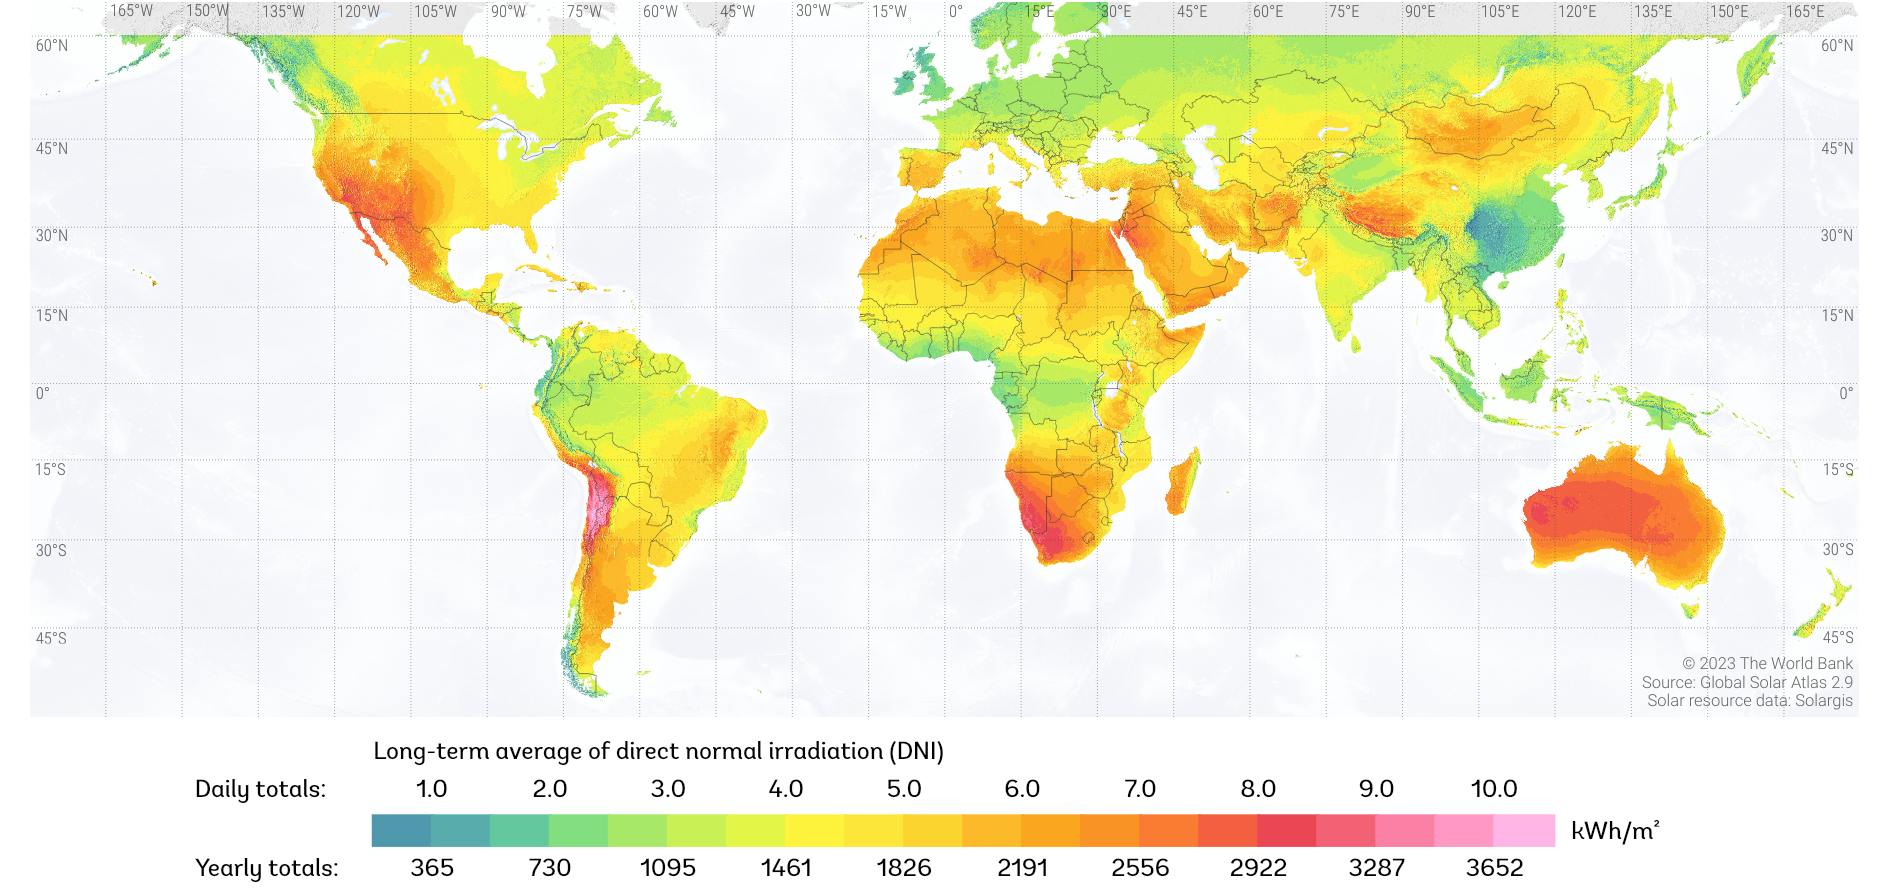
\includegraphics[width=1\textwidth]{img/diseno/dni.png}
    \caption{Mapa mundial del índice de radiación directa normal (\acrshort{dni}) mundial \cite{globalsolar}}
    \label{fig:dni}
\end{figure}

\vspace{3mm}

\begin{figure}[H]
    \centering
    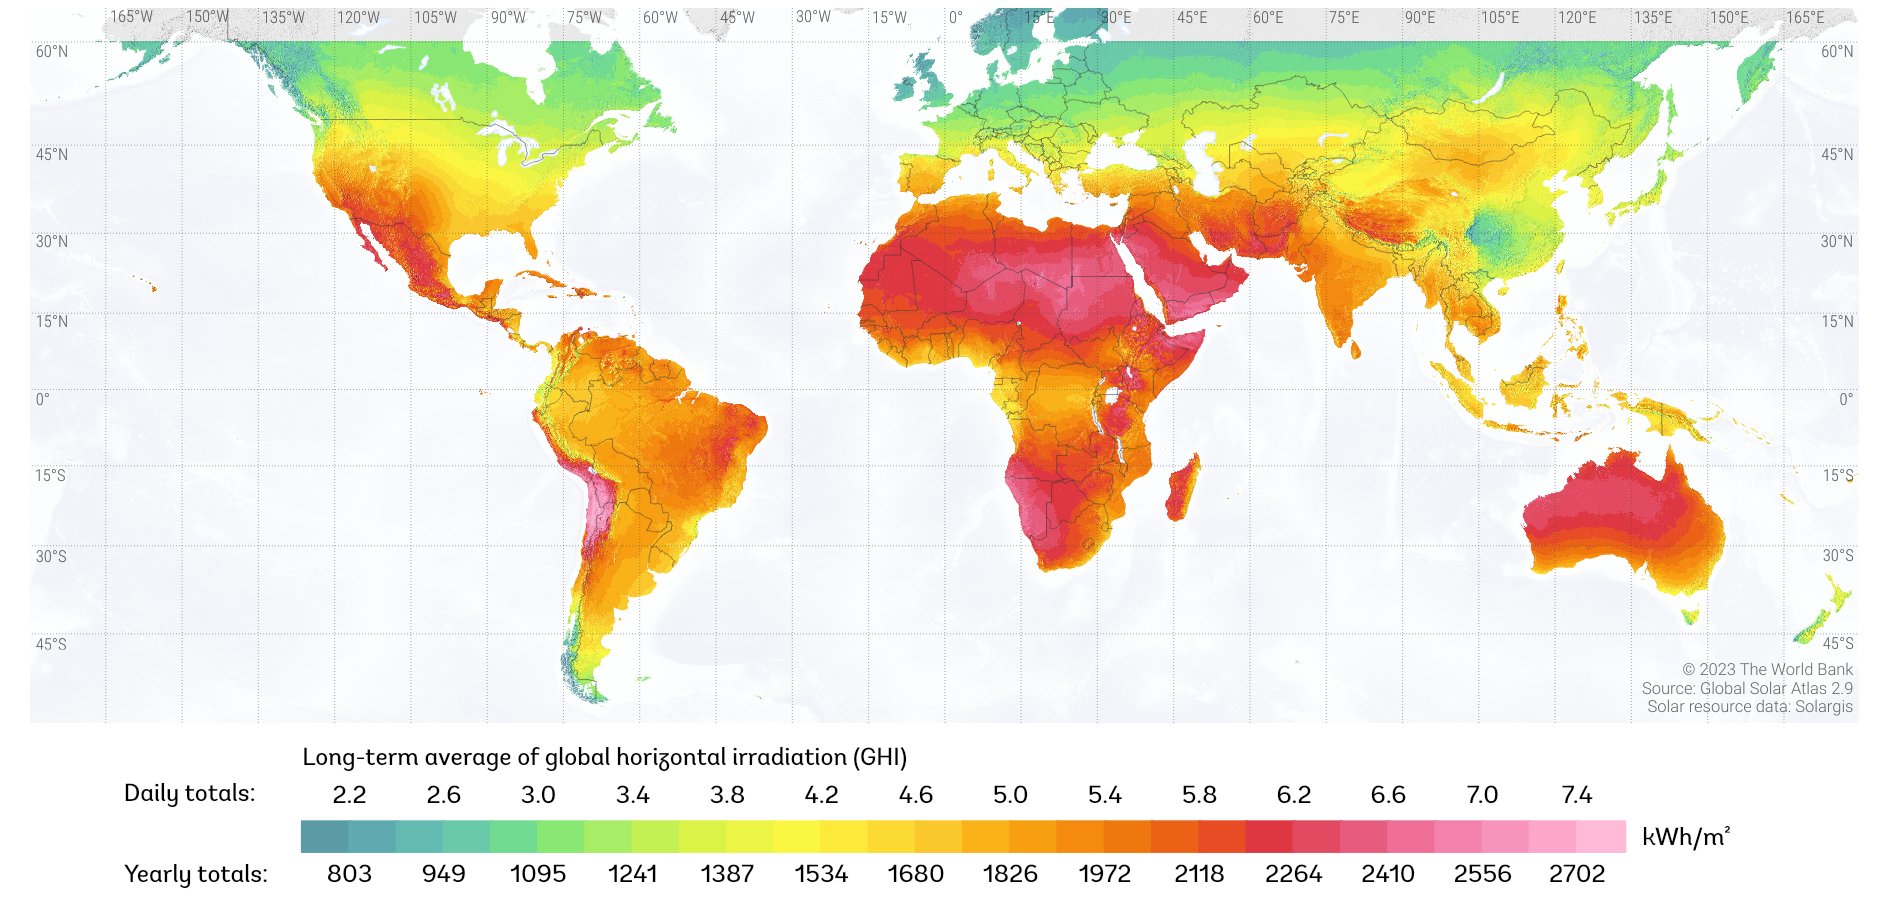
\includegraphics[width=1\textwidth]{img/diseno/ghi.png}
    \caption{Mapa del índice de radiación horizontal global (\acrshort{ghi}) mundial \cite{globalsolar}}
    \label{fig:ghi}
\end{figure}

\vspace{3mm}

\begin{figure}[H]
    \centering
    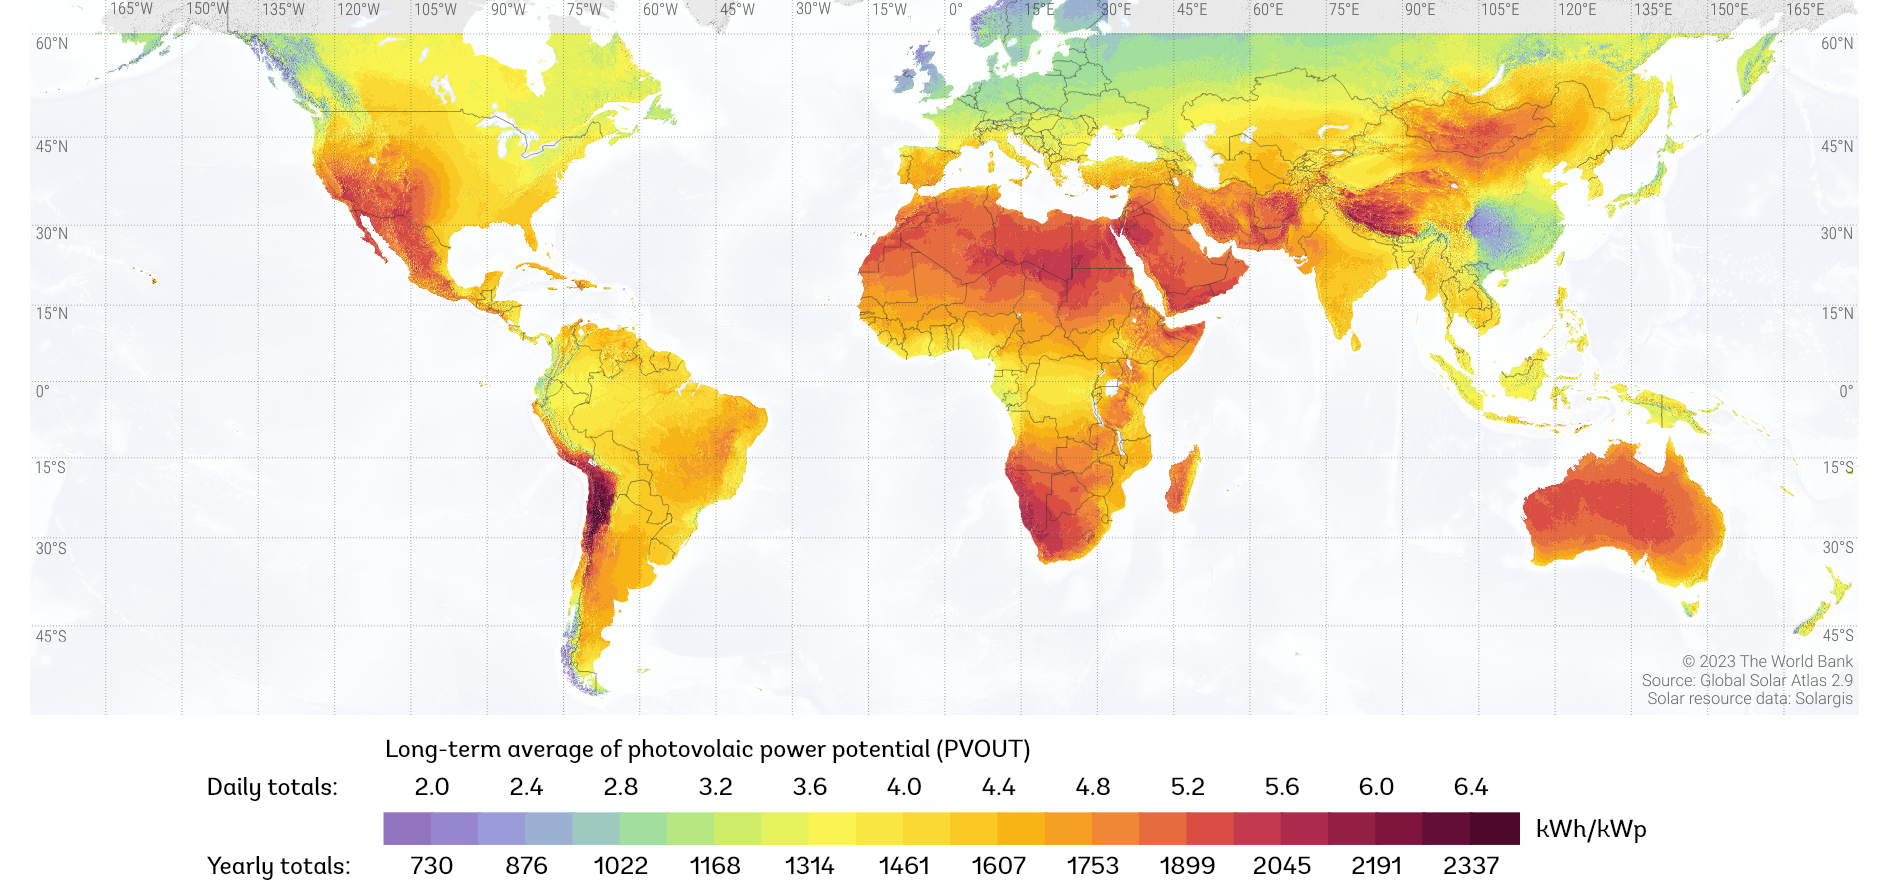
\includegraphics[width=1\textwidth]{img/diseno/photovoltaic.png}
    \caption{Mapa del potencial de producción energética fotovoltaica (\acrshort{pvout}) mundial \cite{globalsolar}}
    \label{fig:photo}
\end{figure}

\subsubsection{Análisis de resultados de radiación}

De la misma forma, lo anterior se hace patente para el caso de la isla de Madeira como se puede visualizar en las Figuras \ref{fig:madeiradni}, \ref{fig:madeiraghi} y \ref{fig:madeirapvout}. Desde la plataforma \textit{Global Solar Atlas} también, se extraen y se recogen en la Tabla \ref{tab:global} los valores de los índices de radiación configurados específicamente para la localización de la ciudad de Funchal. 

\vspace{5mm}

\begin{table}[h!]
    \centering
    \begin{tabular}{|c|c|c|}
    \hline
    \rowcolor[HTML]{AAAAAA} 
    \multicolumn{1}{|c|}{\cellcolor[HTML]{AAAAAA}Parámetro} & \multicolumn{1}{c|}{\cellcolor[HTML]{AAAAAA}kWh/m²/día} & kWh/m²/año \\ \hline
    \gls{dni} & 3,698 & 1349,9 \\ \hline
    \gls{dif} & 2,038 & 743,8 \\ \hline
    \gls{ghi} & 4,345 & 1586,1 \\ \hline
    \gls{gti} & 4,730 & 1726,3 \\ \hline
    \end{tabular}
    \caption{Tabla de valores extraídos para cada índice de radiación en la ciudad de Funchal~\cite{globalsolar}}
    \label{tab:global}
\end{table}

\vspace{3mm}

Por tanto, se puede comprobar a través de estos valores y de la leyenda proporcionada en las figuras anteriores, que Funchal se percibe como una ciudad con un potencial de recursos solares medio alto. Esto es coherente con su localización subtropical y con la elevación del terreno. Es decir, al encontrarse en una zona de costa ronda en valores cercanos a los 100 metros (concretamente 137 metros en la ubicación seleccionada) y se reduce ligeramente el nivel de energía solar captable respecto a otras zonas de la isla más montañosas.

\clearpage

\begin{figure}[H]
    \centering
    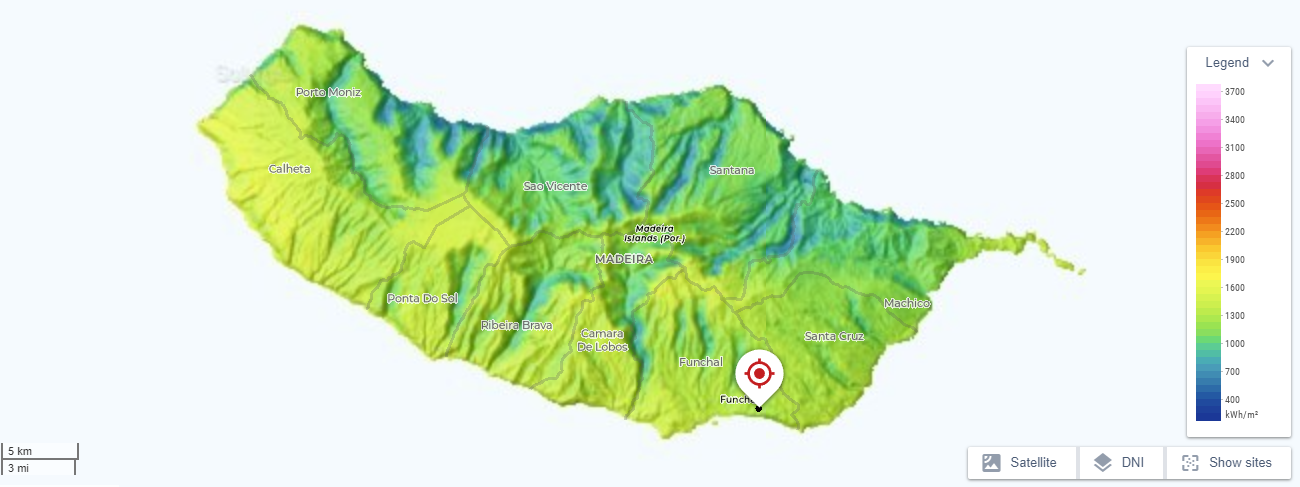
\includegraphics[width=1\textwidth]{img/diseno/madeiradni.png}
    \caption{Mapa del índice de radiación directa normal (\acrshort{dni}) de Madeira \cite{globalsolar}}
    \label{fig:madeiradni}
\end{figure}

\begin{figure}[H]
    \centering
    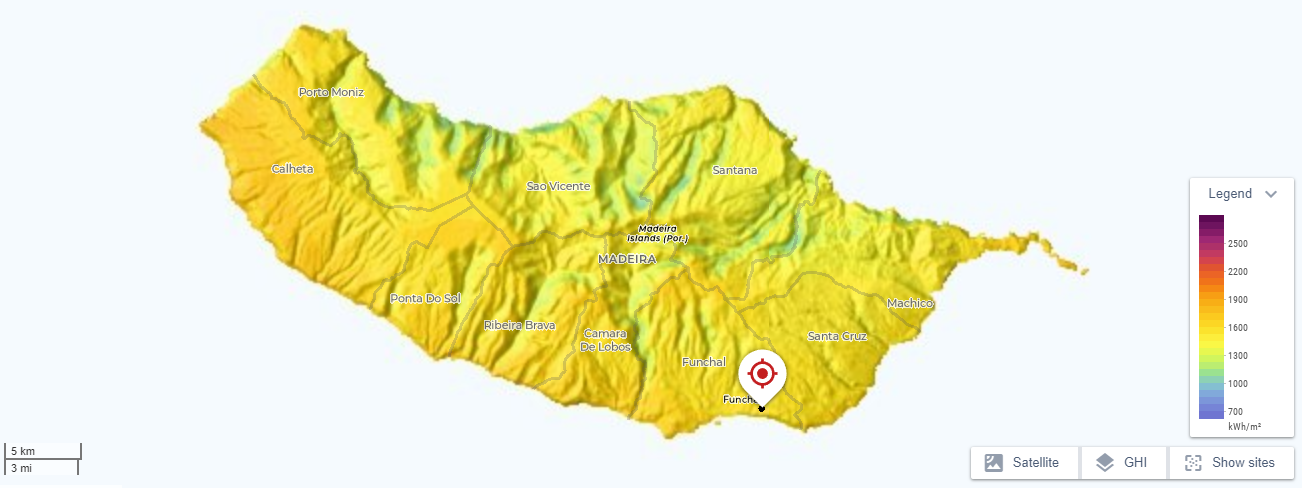
\includegraphics[width=1\textwidth]{img/diseno/madeiraghi.png}
    \caption{Mapa del índice de radiación horizontal global (\acrshort{ghi}) de Madeira \cite{globalsolar}}
    \label{fig:madeiraghi}
\end{figure}

\begin{figure}[H]
    \centering
    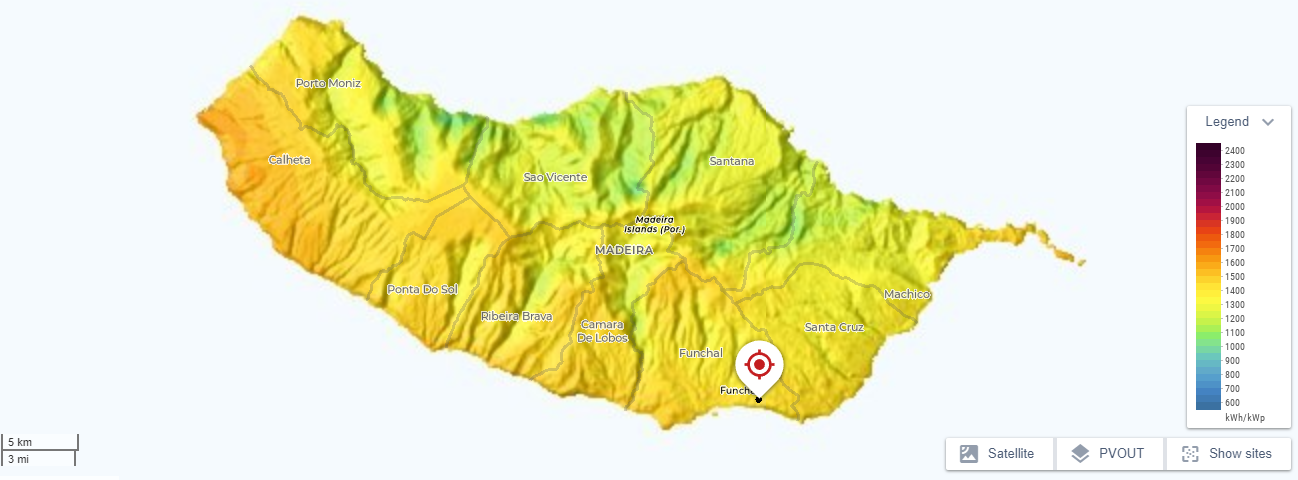
\includegraphics[width=1\textwidth]{img/diseno/madeirapvout.png}
    \caption{Mapa del potencial de producción energética fotovoltaica (\acrshort{pvout}) de Madeira \cite{globalsolar}}
    \label{fig:madeirapvout}
\end{figure}

\pagebreak

\subsubsection{Configuración y cuantificación del potencial energético de la ubicación}

Para calcular de forma aproximada la cantidad de energía que supondría la instalación de un sistema fotovoltaico en la ciudad de Funchal, es preciso configurar primero los siguientes parámetros a través de la plataforma:

\begin{itemize}
    \item Tipo y tamaño de sistema fotovoltaico: Se permite seleccionar entre un sistema enfocado a una vivienda, a un edificio comercial o a una planta solar de grandes dimensiones. En este caso, como se toma como base el estudio de producción energética en un entorno residencial, se configura el primero. Es preciso indicar que en la plataforma la configuración de un sistema fotovoltaico para un entorno residencial no considera la opción de almacenamiento de electricidad.
    \item Capacidad de instalación: Se toma una capacidad máxima de generación de 4kWp (kilovatios pico) para el sistema. En otros términos, este valor determina la cantidad de energía que producirían los paneles en condiciones óptimas.
    \item Azimut \cite{azimut}: Se determina como el ángulo de orientación horizontal y, en función de su valor, define la proyección de los paneles solares en dirección norte, sur, este u oeste. Se indica un valor de 180º para establecer una orientación hacia el sur. 
    \item Inclinación: La plataforma establece como ángulo óptimo para la localización de Funchal un ángulo de 26º, por lo que se configura la instalación de los paneles solares sobre rieles sujetos a un tejado con esta misma inclinación.
\end{itemize}

\subsubsection{Análisis de resultados de potencia}
\label{sec:analisisglobal}

Una vez configurados los parámetros expuestos, se obtienen como resultados la trayectoria solar diaria y los perfiles de radiación y generación fotovoltaica diarios y mensuales para la ubicación de Funchal. En la Figura \ref{fig:azimut} se representa la trayectoria solar diaria, en la que se puede visualizar la comparación de la elevación que percibe el sol en función del instante del año, siendo máxima durante el solsticio de junio, y mínima, durante el de diciembre. En el caso del equinoccio, se sigue una curva con valores promedios, al existir una igualdad entre las horas de día y las de noche. 

\vspace{3mm}

Por otro lado, en la Figura \ref{fig:average} se modelan gráficamente los valores totales mensuales, tanto de producción energética, como de radiación directa normal \gls{dni} para visualizar la correlación existente entre los mismos en los distintos meses del año. El valor promedio máximo energético se alcanza en el mes de julio, con un valor de 565kWh, ocurriendo de la misma forma para el valor máximo de radiación, cuyo alcance es de 163,7kWh/m² para este mes.

\begin{figure}[H]
    \centering
    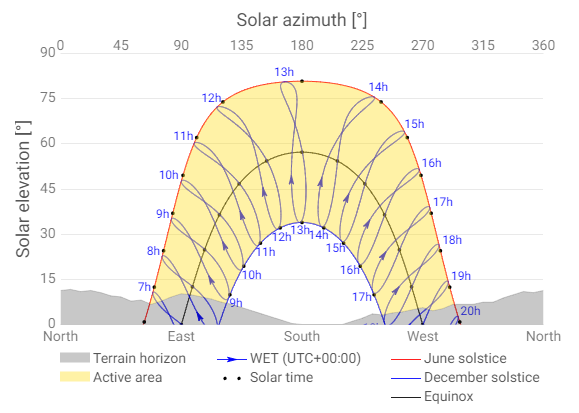
\includegraphics[width=0.85\textwidth]{img/diseno/azimut.png}
    \caption{Representación de la trayectoria solar percibida en la localización de la ciudad de Funchal \cite{globalsolar}}
    \label{fig:azimut}
\end{figure}

\vspace{3mm}

\begin{figure}[H]
    \centering    
    \begin{subfigure}{0.5\linewidth}
        \centering
        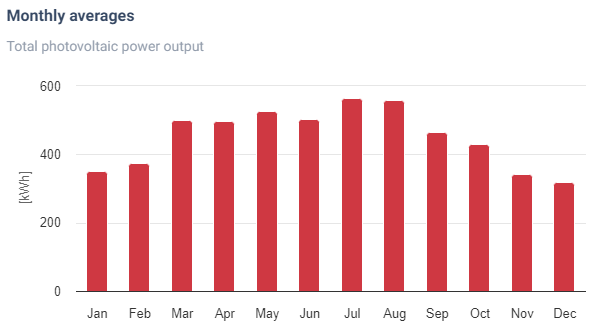
\includegraphics[width=\linewidth,height=5cm]{img/diseno/averagepvout.png}
        \label{fig:averagepvout}
    \end{subfigure}\hfill
    \begin{subfigure}{0.5\linewidth}
        \centering
        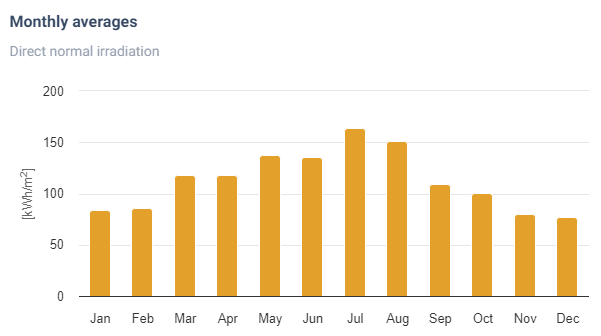
\includegraphics[width=\linewidth,height=5cm]{img/diseno/averagedni.png}
        \label{fig:averagedni}
    \end{subfigure}    
    \caption{Comparación de valores totales mensuales de producción energética fotovoltaica (\acrshort{pvout}) respecto a la radiación directa normal (\acrshort{dni}) \cite{globalsolar}}
    \label{fig:average}
\end{figure}

De la misma forma, se representan en la Figura \ref{fig:averagehour} los perfiles diarios propromedios de radiación y generación fotovoltaica en función del mes del año, en los cuales se encuentran valores máximos en las horas centrales de los meses de julio y agosto. 

\begin{figure}[H]
    \centering    
    \begin{subfigure}{0.75\linewidth}
        \centering
        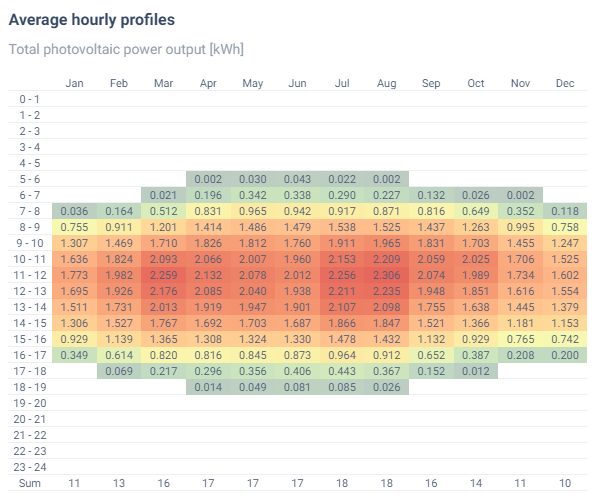
\includegraphics[width=\linewidth]{img/diseno/averagepvouthour.png}
        \label{fig:averagepvouthour}
    \end{subfigure}\hfill

    \begin{subfigure}{0.75\linewidth}
        \centering
        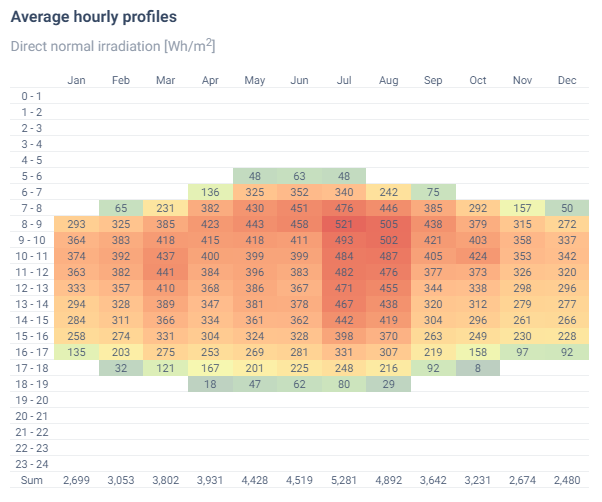
\includegraphics[width=\linewidth]{img/diseno/averagednihour.png}
        \label{fig:averagepdnihour}
    \end{subfigure}    
    \caption{Perfiles promedios de potencial de producción energética fotovoltaica (\acrshort{pvout}) y de radiación directa normal (\acrshort{dni}) \cite{globalsolar}}
    \label{fig:averagehour}
\end{figure}

Tomando en consideración los parámetros configurados y los resultados obtenidos, se puede cuantificar finalmente, que la instalación de un sistema fotovoltaico en un edificio residencial de Funchal proporcionaría una generación de energía promedia anual igual a 5433kWh.

\vspace{3mm}

Este valor viene justificado...

%ver pag 26-31 technical report -> losses


% Total photovoltaic power output and Global tilted irradiation (4)
% 0.015MWh per day 4.711kWh/m2 per day
% 5433kWh per year 1719.4 kWh/m2 per year

% \begin{figure}[H]
%     \centering
%     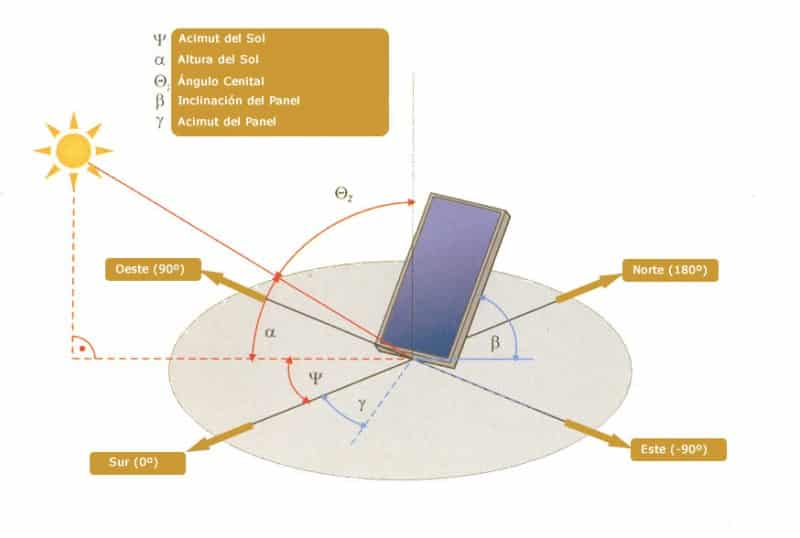
\includegraphics[width=0.8\textwidth]{img/diseno/orient.jpg}
%     \caption{Geometría solar para la instalación de paneles solares \cite{azimut}}
%     \label{fig:orient}
% \end{figure}

% •	Ver pdf PV Systems Performance in Madeira, gráficas interesantes, indica zonas de madeira con mayor producción
% •	Ver Solar Energy Resource in Madeira Islands, gráficas interesantes






\subsection{Creación del dataset de producción (\textit{PVWatts})}
\label{sec:pvw}

Una vez que se han concretado a modo de análisis las características geográficas, climáticas y energéticas de la localización seleccionada en la ciudad de Funchal, se procederá a realizar el paso dedicado a la obtención de los datos de producción fotovoltaica por medio de la simulación. Para ello, se hará uso de la herramienta online \textit{PVWatts}\footnote{https://pvwatts.nrel.gov/pvwatts.php}, proporcionada por el \gls{nrel}, que se trata del laboratorio nacional del Departamento de Energía de Estados Unidos. \cite{pvwatts}

\vspace{3mm}

De la misma forma que se ha operado con la plataforma \textit{Global Solar Atlas} (ver Sección \ref{sec:global}), en el caso de \textit{PVWatts}, también se requiere indicar a la entrada las características relativas a la ubicación seleccionada y a la configuración del sistema de paneles fotovoltaicos que se desea. 

\vspace{3mm}

En cuanto a la primera, la herramienta \textit{PVWatts}, a diferencia de \textit{Global Solar Atlas}, provee un mapa mundial que se rige por celdas, en función de la localización de las bases de datos del \gls{nrel}. En el caso de este \gls{tfm} se cuenta con la fortuna de que se dispone de una de estas bases en la misma ciudad de Funchal, concretamente en las coordenadas 32.65°N, 16.92°W. En este contexto es preciso comentar que esta característica se tuvo en cuenta para definir la localización exacta de instalación del sistema fotovoltaico en la plataforma \textit{Global Solar Atlas} (ver Sección \ref{sec:global}). Por lo tanto, no se requieren ajustes adicionales en estos términos.  

\subsubsection{Configuración de los parámetros de entrada}

Con el objetivo de conseguir a la salida de la simulación unos datos que sean acordes al análisis realizado anteriormente en la Sección \ref{sec:analisisglobal}, es imprescindible replicar y ajustar de la forma más precisa posible los valores de los parámetros de entrada de la herramienta: 

\begin{itemize}
    \item Tamaño del sistema fotovoltaico y capacidad de instalación: Por defecto, \textit{PVWatts} determina una capacidad de 4kWp, por lo que coincide directamente con la definida en \textit{Global Solar Atlas}. Además, se especifica la relación existente entre este valor y el tamaño del sistema de la siguiente manera:
    \[\frac{4 \, \text{kW}}{1 \, \text{kW/m}^2 \times 0.16} = 25 \, \text{m}^2\]
    Donde se representa que, para obtener una eficiencia del 16\% del sistema (eficiencia por defecto), se requiere un área de 25 m² para los módulos solares. Es decir, este valor no representa el área total del sistema fotovoltaico, ya que para ello habría que añadir el cálculo del espacio que se necesita establecer entre cada uno de los paneles DC o el tamaño de los inversores AC que se instalarían.
    \item Índice de cobertura del suelo: Se define como la relación entre el área de superficie del módulo y el área del suelo (tejado en el caso de una vivienda) ocupado en total. El valor predeterminado es de 0.4, lo que supone que, teniendo un área efectiva de 25 m², se necesitará un área total de 62,5 m².
    \item Ratio DC/AC: Haciendo referencia al tamaño de los inversores AC, es preciso exponer que estos limitan la salida de la energía del conjunto para que haya un correcto funcionamiento. La herramienta cuantifica por defecto para la localización, una relación 1.2 entre el tamaño de array de paneles y los inversores de corriente alterna. Por lo tanto, en este caso, estos contarían con una capacidad teórica de 3.33kW. Si se pretendiera realizar una instalación a gran escala se necesitarían ratios de hasta 1.5.
    \item Azimut: De la misma forma que en la configuración en la plataforma \textit{Global Solar Atlas}, se define un azimut de 180º, orientando los paneles hacia el sur.
    \item Inclinación: \textit{Global Solar Atlas}, en el caso de localizar el sistema fotovoltaico en la ciudad de Funchal, establecía como ángulo óptimo de inclinación, un valor de 26º.
    \item Tipo de módulos: Se selecciona el tipo estándar, basado en silicio cristalino y con una cobertura de vidrio con revestimiento antireflectante. Aproximadamente, cuenta con una eficiencia nominal del 19\%.
    \item Tipo de array: Se especifica de forma simplificada un tipo de array fijo, que no siga el movimiento del sol mediante ejes de rotación, sino que mantenga sus valores de inclinación y de azimut configurados. En la Figura \ref{fig:array}, se describe el funcionamiento de cada tipo de array.
\end{itemize}


\begin{figure}[H]
    \centering
    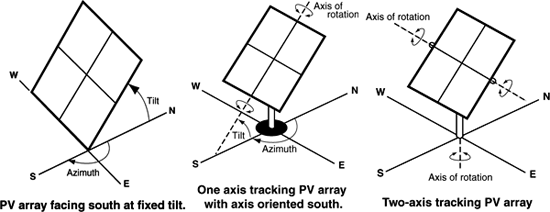
\includegraphics[width=0.85\textwidth]{img/diseno/array.png}
    \caption{Representación de las diferentes opciones de array que permite configurar la herramienta \textit{PVWatts} \cite{pvwatts}}
    \label{fig:array}
\end{figure}

\subsubsection{Configuración de las pérdidas del sistema real}

Una de las ventajas de uso que permite la herramienta \textit{PVWatts} es la posibilidad de estimar las pérdidas totales que tendría el sistema en la realidad. Esto es importante para que los resultados de la simulación que se va a realizar sean lo más parecidos a los que se obtendrían mediante la medición del sistema real. Para ello, se deben configurar cada una de las pérdidas parciales de la siguiente manera:

\begin{itemize}
    \item Suciedad: Debido a la escasez de precipitaciones y a la presencia de calima que se experimenta en la isla, se determina un valor de un 2\%.
    \item Sombreado: Se reduce la radiación solar que incide en los paneles si se producen sombras por objetos cercanos o por la propia de los módulos si se colocan en fila. Es decir, estos crean sombras sobre los de la fila adyacente. El cálculo se realiza a partir de la gráfica expuesta en la Figura \ref{fig:sombra}. Por lo tanto, como se ha definido un tipo de array fijo con una inclinación de 26º y un valor de índice de cobertura del suelo de 0.4, se determina aproximadamente un valor de pérdidas por sombra igual a un 3\%.
    \item Nieve: Teniendo en cuenta las características climáticas de la ciudad de Funchal debido a su localización en una zona subtropical, se determinan pérdidas del 0\%.
    \item Discordancia: Son pérdidas eléctricas debido a las diferencias que se producen por imperfecciones en la fabricación de los módulos. Esto tiene como consecuencia que cada uno de ellos presente características I-V que varíen ligeramente entre sí. La herramienta proporciona un valor predeterminado del 2\%.
    \item Cableado y conexiones: Pérdidas resistivas en el cableado y en las conexiones entre módulos, inversores y otros elementos del sistema con un valor por defecto del 2\% y del 0.5\%, respectivamente.
    \item Degradación inducida por la luz: Se trata del efecto de reducción de potencia que se produce durante los primeros meses de funcionamiento del sistema fotovoltaico. El valor predeterminado es 1,5\%.
    \item Precisión del fabricante: Son pérdidas, generalmente bajas, que vienen definidas por la precisión del fabricante en el proceso de estudio de eficiencia de los paneles. Se determina un 1\%.
    \item Disponibilidad: Se añaden las pérdidas que se producen a partir de los mantenimientos que se requieren a lo largo del tiempo y que causan paradas en el funcionamiento del sistema. Se provee un valor por defecto del 3\%.
\end{itemize}

Finalmente, las pérdidas totales del sistema se pueden cuantificar a partir de la siguiente expresión:
    \[\textit{Losses} = (1-0.02) \times (1-0.03) \times (1-0.02) \times (1-0.02) 
    \times (1-0.005) \times (1-0.015) \times (1-0.01) \times (1-0.03)\]
    \[100\% \times (1-\textit{Losses}) = 14,08\%\]

\begin{figure}[H]
    \centering
    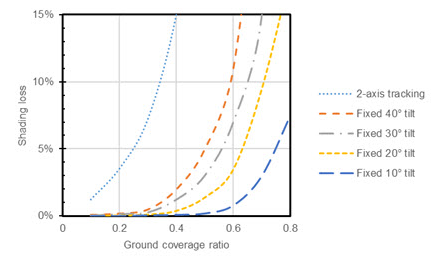
\includegraphics[width=0.8\textwidth]{img/diseno/sombra.png}
    \caption{Gráfica para el cálculo de las pérdidas por sombreado en la herramienta \textit{PVWatts}~\cite{pvwatts}}
    \label{fig:sombra}
\end{figure}

\subsubsection{Análisis de resultados de la simulación}

Una vez se ha concluido con la configuración necesaria, se procede a ejecutar la simulación en la herramienta y a adquirir a la salida los resultados de la misma. Se obtienen dos datasets que replican un año completo de mediciones: uno con los valores totales mensuales (ver Tabla \ref{tab:pvwattsdataset2}) y otro, con un conjunto de muestras que proporcionan información de cada hora (ver Tabla \ref{tab:pvwattsdataset}). 

\vspace{3mm}

%%AQUI HABLAR DE LOS PARAMETROS QUE SE DAN

\begin{table}[h!]
    \centering
    \begin{tabular}{|c|c|c|}
    \hline
    \rowcolor[HTML]{AAAAAA} 
    \multicolumn{1}{|c|}{\cellcolor[HTML]{AAAAAA}Campo} & \multicolumn{1}{c|}{\cellcolor[HTML]{AAAAAA}Descripción} & Unidades \\ \hline
    \textit{Month} & Mes de la muestra & - \\ \hline
    \textit{Daily POA Irradiance} & Índice de radiación en el plano del array & kWh/m2/day \\ \hline 
    \textit{DC Array Output} & Potencia de salida DC del array & kWh \\ \hline
    \textit{AC System Output} & Potencia de salida AC del sistema & kWh \\ \hline
    \end{tabular}
    \caption{Dataset con valores totales mensuales \cite{pvwatts}}
    \label{tab:pvwattsdataset2}
\end{table}

\vspace{3mm}

\begin{table}[h!]
    \centering
    \begin{tabular}{|c|c|c|}
    \hline
    \rowcolor[HTML]{AAAAAA} 
    \multicolumn{1}{|c|}{\cellcolor[HTML]{AAAAAA}Campo} & \multicolumn{1}{c|}{\cellcolor[HTML]{AAAAAA}Descripción} & Unidades \\ \hline
    \textit{Month} & Mes de la muestra & - \\ \hline
    \textit{Day} & Día de la muestra & - \\ \hline
    \textit{Hour} & Hora de la muestra & - \\ \hline
    \textit{Beam Irradiance} & Índice de radiación directa normal (\gls{dni}) & W/m2 \\ \hline %%%%%%%%%%
    \textit{Diffuse Irradiance} & Índice de radiación difusa (\gls{dif}) & W/m2 \\ \hline
    \textit{Plane of Array Irradiance} & Índice de radiación en el plano del array & W/m2 \\ \hline %%%%%%%%%%
    \textit{Ambient Temperature} & Temperatura ambiente & C \\ \hline
    \textit{Wind Speed} & Velocidad del viento & m/s \\ \hline
    \textit{Albedo} & Índice de reflectividad de la superficie & - \\ \hline
    \textit{Cell Temperature} & Temperatura de las células solares & C \\ \hline
    \textit{DC Array Output} & Potencia de salida DC del array & W \\ \hline
    \textit{AC System Output} & Potencia de salida AC del sistema & W \\ \hline
    \end{tabular}
    \caption{Dataset con muestras adquiridas por hora \cite{pvwatts}}
    \label{tab:pvwattsdataset}
\end{table}

\vspace{3mm}

En este paso, es imprescindible comprobar que los datos finales obtenidos presentan coherencia respecto al estudio previo y que encajan además, con el análisis de los resultados de la plataforma \textit{Global Solar Atlas}, realizado en la Sección \ref{sec:analisisglobal}. 

\vspace{3mm}

En primera instancia, se va a proceder a poner el foco en los valores de radiación directa normal \gls{dni}. La herramienta \textit{PVWatts}, como se puede ver en la Tabla \ref{tab:pvwattsdataset2}, no proporciona directamente información mensual sobre este parámetro, sino sobre el índice de radiación en el plano del array (del inglés \gls{poa}), que se calcula a partir de la expresión \cite{poa}:

\[ \gls{poa} = \gls{dni} \cdot \cos(\theta) \]

    Donde:
\begin{itemize}
    \renewcommand{\labelitemi}{}
    \item \( \theta \) es el ángulo de inclinación configurado, que en este caso sería de 26º.
\end{itemize}

\vspace{3mm}

Por tanto, se pueden calcular los valores de \gls{dni} a partir de los de \gls{poa} dados por el dataset. En la Figura \ref{fig:averagereal} se pueden observar los valores totales mensuales, tanto de producción energética, como de radiación directa normal \gls{dni}. El valor máximo energético se alcanza en el mes de julio, con un valor de 517,8kWh, ocurriendo de la misma forma para el valor promedio máximo de radiación, cuyo alcance es de 181.1kWh/m² para este mes. Por tanto, volviendo a la Sección \ref{sec:analisisglobal} y, específicamente a la \ref{fig:average}, se puede determinar que los valores obtenidos en la simulación son muy precisos respecto al estudio previo.

\vspace{3mm}

\begin{figure}[H]
    \centering    
    \begin{subfigure}{0.5\linewidth}
        \centering
        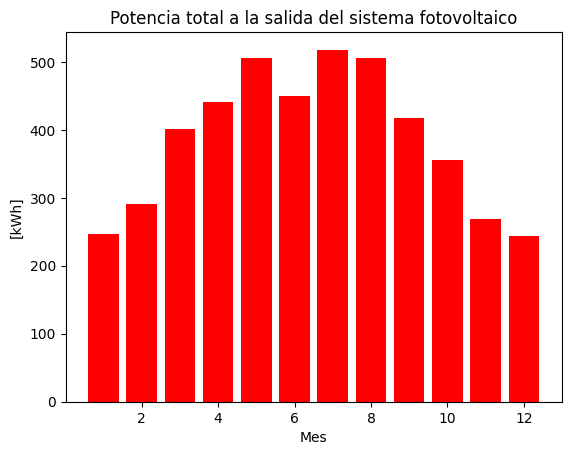
\includegraphics[width=\linewidth,height=6.5cm]{img/diseno/averagepvoutreal.png}
        \label{fig:averagepvoutreal}
    \end{subfigure}\hfill
    \begin{subfigure}{0.5\linewidth}
        \centering
        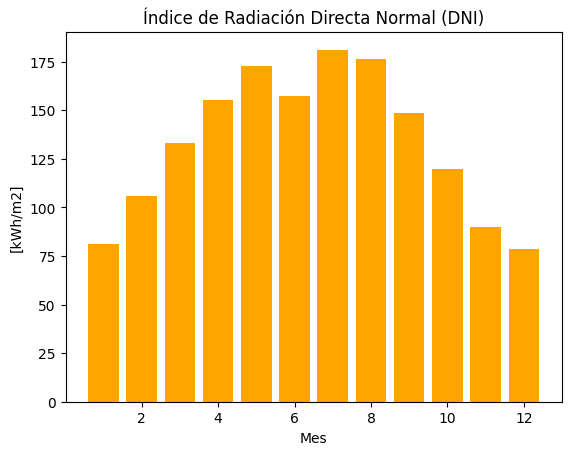
\includegraphics[width=\linewidth,height=6.5cm]{img/diseno/averagednireal.png}
        \label{fig:averagednireal}
    \end{subfigure}    
    \caption{Comparación de valores totales mensuales de producción energética fotovoltaica (\acrshort{pvout}) respecto a la radiación directa normal (\acrshort{dni}) a partir de los resultados de la simulación}
    \label{fig:averagereal}
\end{figure}

Aparte de las gráficas realizadas, se expone la Tabla \ref{tab:globalvspvwatts} para llevar a cabo de una forma correcta la comparación entre los valores estudiados en \textit{Global Solar Atlas} y los resultantes de la simulación en \textit{PVWatts}. Como se puede ver, existe un menor error entre los valores respectivos a la radiación que entre los valores de potencia producida. Las diferencias percibidas provienen principalmente por las pérdidas configuradas, ya que al final los resultados de la simulación son mucho más cercanos al caso real que los percibidos teóricamente. 

\begin{sidewaystable}
    \centering 
    \begin{tabularx}{\textheight}{|c|XX|XX|}
        \hline
        \rowcolor[HTML]{EFEFEF} 
        \cellcolor[HTML]{C0C0C0} & \multicolumn{2}{c|}{\cellcolor[HTML]{C0C0C0}Producción energética fotovoltaica (PVOUT) [kWh]} & \multicolumn{2}{c|}{\cellcolor[HTML]{C0C0C0}Índice de Radiación Directa Normal (DNI) [kWhm2]} \\ \cline{2-5} 
        \rowcolor[HTML]{C0C0C0} 
        \multirow{-2}{*}{\cellcolor[HTML]{C0C0C0}Mes} & \multicolumn{1}{c|}{\cellcolor[HTML]{C0C0C0}Global Solar Atlas} & PVWatts & \multicolumn{1}{c|}{\cellcolor[HTML]{C0C0C0}Global Solar Atlas} & PVWatts \\ \hline
        \textit{Enero} & \multicolumn{1}{c|}{350,2} & \multicolumn{1}{c|}{247,1} & \multicolumn{1}{c|}{83,7} & \multicolumn{1}{c|}{81,1} \\ \hline
        \textit{Febrero} & \multicolumn{1}{c|}{374,0} & \multicolumn{1}{c|}{291,4} & \multicolumn{1}{c|}{85,5} & \multicolumn{1}{c|}{105,7} \\ \hline
        \textit{Marzo} & \multicolumn{1}{c|}{500,8} & \multicolumn{1}{c|}{401,9} & \multicolumn{1}{c|}{117,9} & \multicolumn{1}{c|}{132,8} \\ \hline
        \textit{Abril} & \multicolumn{1}{c|}{497,9} & \multicolumn{1}{c|}{441,3} & \multicolumn{1}{c|}{117,9} & \multicolumn{1}{c|}{155.0} \\ \hline
        \textit{Mayo} & \multicolumn{1}{c|}{526,5} & \multicolumn{1}{c|}{505,9} & \multicolumn{1}{c|}{137,3} & \multicolumn{1}{c|}{172.7} \\ \hline
        \textit{Junio} & \multicolumn{1}{c|}{502,5} & \multicolumn{1}{c|}{449,6} & \multicolumn{1}{c|}{135,6} & \multicolumn{1}{c|}{157.4} \\ \hline
        \textit{Julio} & \multicolumn{1}{c|}{565,5} & \multicolumn{1}{c|}{517,8} & \multicolumn{1}{c|}{163,7} & \multicolumn{1}{c|}{181.1} \\ \hline
        \textit{Agosto} & \multicolumn{1}{c|}{558,6} & \multicolumn{1}{c|}{505,5} & \multicolumn{1}{c|}{151,6} & \multicolumn{1}{c|}{176.1} \\ \hline
        \textit{Septiembre} & \multicolumn{1}{c|}{465,3} & \multicolumn{1}{c|}{417,4} & \multicolumn{1}{c|}{109,3} & \multicolumn{1}{c|}{148.7} \\ \hline
        \textit{Octubre} & \multicolumn{1}{c|}{429,0} & \multicolumn{1}{c|}{356,3} & \multicolumn{1}{c|}{100,2} & \multicolumn{1}{c|}{119.5} \\ \hline
        \textit{Noviembre} & \multicolumn{1}{c|}{343,7} & \multicolumn{1}{c|}{268,8} & \multicolumn{1}{c|}{80,2} & \multicolumn{1}{c|}{90,1} \\ \hline
        \textit{Diciembre} & \multicolumn{1}{c|}{318,6} & \multicolumn{1}{c|}{243,4} & \multicolumn{1}{c|}{76,9} & \multicolumn{1}{c|}{78,6} \\ \hline
    \end{tabularx}
    \caption{Tabla de comparación de los valores totales mensuales de producción energética fotovoltaica (\acrshort{pvout}) y de radiación directa normal (\acrshort{dni}) de las dos herramientas (valores teóricos y simulados)}
    \label{tab:globalvspvwatts}
\end{sidewaystable}


\vspace{3mm}

Por lo tanto, a través del sumatorio de todos los valores mensuales de producción energética, se puede cuantificar finalmente, que un sistema fotovoltaico real localizado en la ciudad de Funchal, proveería aproximadamente un total de 4417kWh al año. Este valor representa un 81,3\% del obtenido teóricamente en la Sección \ref{sec:analisisglobal} y viene justificado en gran parte por las pérdidas introducidas. 

\vspace{3mm}

Adicionalmente, habría que tener en cuenta las diferencias que presentan las herramientas \textit{Global Solar Atlas} y \textit{PVWatts} en sus algoritmos de cálculo de los valores de potencia, ya que cada una de ellas asignará pesos diferentes a los parámetros de entrada, incidiendo en los resultados. No obstante, con la Tabla \ref{tab:globalvspvwatts}, se puede determinar de forma concluyente que la simulación realizada es coherente con el estudio previo, cumpliendo así el objetivo principal de esta Sección.

\clearpage 

% %%%%%%%%%%%%%%%%%%%%%%%%%%%%%%%%%%%%%%%%%%%%%%%%%%%%%%%%%%%%%%%%%%%%%%%%%%%%%%%%%%%%%%%%%%%%%%%%%
%%%%%%%%%%%%%%%%%%%%%%%%%%%%%%%%%%%%%%%%%%%%%%%%%%%%%%%%%%%%%%%%%%
\section{Preprocesado}
\label{sec:preprocesado}

% %%%%%%%%%%%%%%%%%%%%%%%%%%%%%%%%%%%%%%%%%%%%%%%%%%%%%%%%%%%%%%%%%%%%%%%%%%%%%%%%%%%%%%%%%%%%%%%%%
%%%%%%%%%%%%%%%%%%%%%%%%%%%%%%%%%%%%%%%%%%%%%%%%%%%%%%%%%%%%%%%%%%
\section{Planteamiento de escenarios y generación de topologías en \acrshort{brite}}
\label{sec:ejebrite}

La presente Sección está dedicada al planteamiento de una serie de escenarios de red y a la consecuente generación de topologías mediante el empleo de la herramienta \gls{brite}, cuyo funcionamiento ha sido descrito en la Sección \ref{sec:brite}. La importancia de esta fase del diseño viene dada por la necesidad de aplicar la operativa del algoritmo \gls{den2ne} sobre múltiples topologías para obtener, finalmente, el dataset sobre el que se entrenarán y desarrollarán los modelos de \gls{ml} y \gls{dl}. Se debe tener en cuenta que, para que este conjunto de datos final permita aportar suficiente información útil a los modelos, el número de topologías aleatorias a generar en \gls{brite} debe de ser relativamente elevado.

\vspace{3mm}

\subsection{Planteamiento de escenarios y configuración de \acrshort{brite}}
\label{sec:conftopo}

Para emplear la herramienta, se deben plantear los escenarios de red sobre los que se desea basar la generación de topologías aleatorias. Por ello, es preciso definir la configuración de los parámetros de entrada en el script \textit{autogenerador.sh}, tomando en consideración el requerimiento anterior. Como se especificaba en la Sección \ref{sec:brite_eje}, este script está dedicado a la automatización de la ejecución, tanto de la herramienta, como del \textit{parser}, para obtener a la salida los ficheros finales con las posiciones de los nodos en el plano y con la información relativa a las distancias y a los nodos que se interconectan con cada enlace (\textit{Nodos.txt} y \textit{Enlaces.txt}). 

\vspace{3mm}

Entonces, se puede expresar que el cálculo del número total de topologías que se pueden generar con \gls{brite} resultará de operar el producto de los siguientes parámetros de entrada configurados:

\begin{itemize}
    \item Número de modelos de topología a emplear: Como se había introducido en la Sección \ref{sec:modelostopos}, este \gls{tfm} se va a basar en el empleo de topologías aleatorias a nivel de router y, en particular, en los modelos Router Waxman y Router Barabasi-Albert. 
    \item Número de dimensiones: Para las pruebas a simular en el algoritmo \gls{den2ne}, se pretende manejar topologías con una gran cantidad de nodos, pero reduciendo los saltos de incremento del total. Por ello, se configura una generación desde 100 a 200 nodos con un incremento de 50 en 50, suponiendo la configuración de 3 dimensiones de topologías (100, 150 y 200 nodos). 
    \item Número de grados de conectividad: Este parámetro determina el número de enlaces por nodo y se especifican 3 grados \textit{m} diferentes en el script. Es preciso indicar que, como en \gls{den2ne} se tratarán los enlaces como bidireccionales, realmente cada topología tendrá un grado \textit{2m}.
    \item Número de semillas de generación: Es importante destacar que para la generación de topologías aleatorias se aplican 10 ficheros de semillas. Esto tiene como resultado la generación de 10 topologías diferentes para cada uno de los escenarios configurados o, en otros términos, para cada una de las configuraciones posibles de los parámetros de entrada.
\end{itemize}

\vspace{3mm}

Adicionalmente, se deben determinar otros parámetros que hacen referencia a los nodos, como son el modo de introducción al plano y su posicionamiento. Respectivamente, se establece una introducción incremental y un posicionamiento totalmente aleatorio alrededor del plano. También, los parámetros específicos del modelo Router Waxman, $\alpha$ y $\beta$, que toman valores de 0,2 y 0,15, respectivamente.

\vspace{3mm}

\begin{lstlisting}[language=bash, style=Consola, caption={Configuración de los parámetros de entrada en el script de automatización de \acrshort{brite}}]
topologia_rt_waxman=1  # Empleo de modelo RTWaxman
topologia_rt_barabasi=2  # Empleo de modelo RTBarabasi
nodos=$(seq 100 50 200) # Número de nodos por topología (dimensiones)
m=(1 2 3) # El grado de conectividad real es 2, 4, 6
n_topologias_distintasxnodo=10 # Número de topologías aleatorias en función del número de semillas

NodePlacement=1 # Posicionamiento aleatorio de los nodos
GrowthType=1 # Modo de introducción incremental

#parametros especificos de Waxman
alpha=0.2
beta=0.15
\end{lstlisting}

\subsection{Resultados de la generación de topologías aleatorias}
\label{sec:gentopo}

Considerando los parámetros de entrada configurados anteriormente, se puede cuantificar el número total de topologías que resultará de la ejecución del script \textit{autogenerador.sh} a partir de la siguiente expresión:

    \[\textit{N\_topos} = \textit{Nmodelos} \times \textit{Ndimensiones}
    \times \textit{Ngrados} \times \textit{Nseeds\_gen}\]
    \[\textit{N\_topos} = 2 \times 3 \times 3 \times 10 = 180\]

\vspace{3mm}

Es preciso indicar que en el caso de requerirse un mayor número de topologías a simular en \gls{den2ne}, bastaría únicamente con modificar el rango establecido para el número de nodos o el valor del incremento de los mismos. No obstante, puesto que se pretende tener en cuenta para la ejecución del algoritmo el dataset resultante de la etapa de procesamiento (ver Sección \ref{sec:combinacion}), no se precisa aumentar el número de topologías aleatorias a priori. Estos motivos vendrán justificados detalladamente en la Sección \ref{sec:confden2ne}, dedicada a la configuración de los parámetros de entrada de \gls{den2ne}.

\vspace{3mm}

De forma adicional, para observar gráficamente los resultados que se obtienen a la salida se representan varios ejemplos de topologías generadas en la Figura \ref{fig:grafbrite}. Respectivamente, las gráficas obtenidas de \textit{matlab} hacen referencia al modelo Barabasi-Albert y al Waxman y presentan una configuración de 100 nodos y un grado de conectividad \textit{m}=2, que al suponer enlaces direccionales realmente toma el valor de 4. Es importante indicar que, para apreciar las diferencias existentes entre ambos modelos, se selecciona el mismo fichero de semilla (\textit{seed\_4}) para la representación.

\vspace{3mm}

\begin{figure}[h!]
    \centering
    \begin{minipage}{0.5\textwidth}
      \centering
      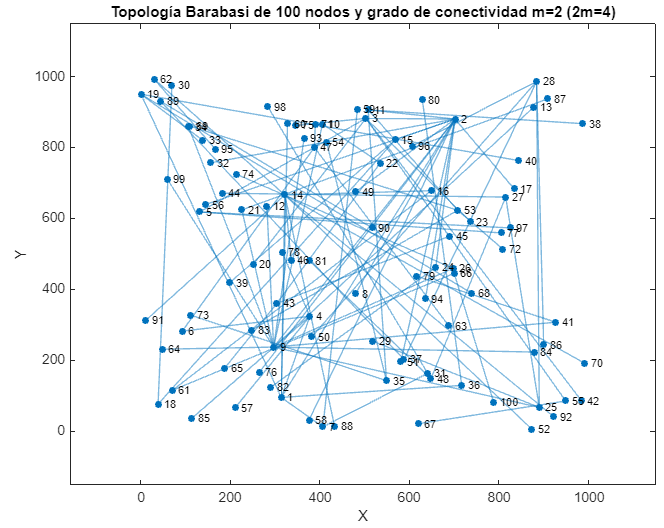
\includegraphics[width=\linewidth]{img/diseno/britebarabasi2.png}
      \label{fig:grafbrite1}
    \end{minipage}\hfill
    \begin{minipage}{0.5\textwidth}
      \centering
      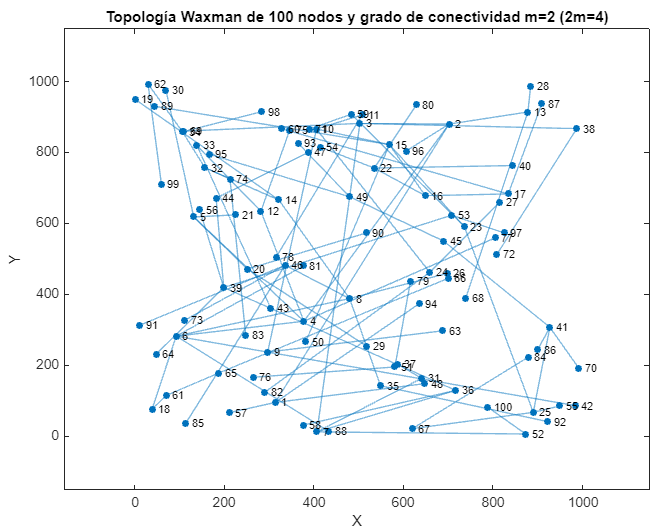
\includegraphics[width=\linewidth]{img/diseno/britewaxman2.png}
      \label{fig:grafbrite2}
    \end{minipage}\hfill
    \caption{Representación de diferencias de los modelos Router Barabasi-Albert y Waxman a partir de los mismos parámetros de entrada}
    \label{fig:grafbrite}
\end{figure}

% %%%%%%%%%%%%%%%%%%%%%%%%%%%%%%%%%%%%%%%%%%%%%%%%%%%%%%%%%%%%%%%%%%%%%%%%%%%%%%%%%%%%%%%%%%%%%%%%%
%%%%%%%%%%%%%%%%%%%%%%%%%%%%%%%%%%%%%%%%%%%%%%%%%%%%%%%%%%%%%%%%%%
\section{Simulación de las topologías en \acrshort{den2ne}}

Esta Sección viene dada por el objetivo de obtener el conjunto de datos final sobre el que se basará el desarrollo en el Capítulo \ref{cha:desarrollo}. Para lograrlo, se requiere llevar a cabo un gran número de  simulaciones en \gls{den2ne} a partir de las topologías generadas con la herramienta \gls{brite} (ver Sección \ref{sec:ejebrite}). 

\vspace{3mm}

No obstante, previamente a la ejecución del algoritmo, es imprescindible implementar una serie de modificaciones en el mismo para ajustar su funcionamiento para obtener resultados de utilidad para el presente \gls{tfm}. La secuencia de acciones que se llevará a cabo se detallará en la Sección \ref{sec:cambiosden2ne}. De la misma forma, se justificará el criterio escogido para determinar cúando se producen errores en el proceso de distribución energética. Esto servirá de base para después entrenar los modelos de \gls{ml} y \gls{dl}.

\vspace{3mm}

Por consiguiente, se añade la Sección \ref{sec:confden2ne}, donde se especificará la configuración de los parámetros de entrada de \gls{den2ne} y se cuantificará el número total de pruebas posibles que se podrían llegar a realizar a partir de las topologías generadas y de los datos reales procesados anteriormente. Se comprobará a través de diferentes pruebas que las modificaciones introducidas en el algoritmo \gls{den2ne} producen una operativa acorde a las necesidades de este \gls{tfm}. De forma concluyente, a partir de los resultados obtenidos en las simulaciones, se añadirá la Sección \ref{sec:datasetfinal}, en referencia a las características del dataset final que se utilizará para el entrenamiento de los modelos.

\subsection{Adaptación del algoritmo \acrshort{den2ne} a las pruebas}
\label{sec:cambiosden2ne}

Todas las modificaciones realizadas en el funcionamiento del algoritmo \acrshort{den2ne} han sido aplicadas a partir de los ficheros contenidos en el repositorio\footnote{https://github.com/NETSERV-UAH/den2ne-Alg} del equipo de investigación NetIS de la \gls{uah}.

\subsubsection{Importación de los perfiles de carga reales}
\label{sec:importcarga}

La primera modificación que se debe implementar en el funcionamiento de \gls{den2ne} consiste en la importación de los valores de carga reales, obtenidos como resultado de llevar a cabo la fase de procesamiento de los datos (ver Sección \ref{sec:combinacion}). La necesidad de aplicar este paso se debe a que el algoritmo, a partir de una topología dada a la entrada, establece una función de densidad de probabilidad para determinar de forma aleatoria un valor de carga para cada uno de los nodos de una topología. Para modificar este proceso se sigue la siguiente secuencia de pasos:

\begin{enumerate}
    \item Definición de función \textit{getLoads\_Config} en \textit{dataCollector.py}: Se añade una función de recolección de las configuraciones de carga reales, pasando como argumentos el directorio definido en \textit{path\_simtests} y el fichero de pruebas \textit{sim\_file}. Después, se inicializa una variable de diccionario y se almacenan los valores de potencia generada, consumida y la diferencia calculada de ambas. Estos valores se manejan en términos de kW, puesto que \gls{den2ne} está configurado para trabajar en esta unidad.
    \item Definición de funciones \textit{cargas} y \textit{cargas\_con\_limite} en \textit{brite\_intf.py}: Ambas funciones se encargan de aplicar los valores de carga reales, extraídos de la función anterior, a cada uno de los nodos de una topología determinada. En el caso de las simulaciones que se realizan en este \gls{tfm}, se hará uso de la primera, debido a que no se configuran límites de los valores de carga (ver Sección \ref{sec:confden2ne}). Por tanto, poniendo el foco en la función \textit{cargas}, se pasa como argumento el diccionario resultante de la función \textit{getLoads\_Config} y se extrae a partir de las claves del mismo el número de perfiles de carga (23) a manejar. De la misma forma, se pasa también como argumento el fichero de nodos, anteriormente generado con \gls{brite} y el \textit{parser}, para conocer las dimensiones que tiene la topología en cuestión. Con este dato se determina la cantidad de iteraciones que son necesarias para aplicar el valor de carga real a todos los nodos de una topología y, para cada uno de ellos, se determina de forma aleatoria uno de los 23 perfiles reales de carga. A la salida, se obtiene un nuevo diccionario con tamaño igual al número de nodos que hay en la topología y que viene constituido por la información del identificador del perfil real seleccionado y del valor de carga neta aplicada.
    \item Definición de la variable \textit{id\_orig} en \textit{node.py}: Se añade al constructor de la clase de nodo que tiene \gls{den2ne} un nuevo elemento, en relación al identificador del perfil de carga seleccionado para un nodo en cuestión.
    \item Introducción de la variable \textit{id\_orig} en la función \textit{buildGraph} en \textit{graph.py}: La nueva variable de nodo se incluye en el proceso de generación del grafo para mantener el conocimiento del perfil de carga que se ha seleccionado para cada nodo durante la ejecución completa del algoritmo.
    \item Modificaciones en \textit{test\_topo.py}: El fichero dedicado a las pruebas de \gls{den2ne} debe incluir las llamadas a las funciones creadas o modificadas anteriormente. También, requiere definir los nuevos parámetros \textit{path\_simtests} y \textit{sim\_file}, en referencia a los ficheros de prueba que contienen los valores de carga, extraídos del dataset para un instante temporal determinado (ver Sección \ref{sec:datasetfinal}).
\end{enumerate} 

\subsubsection{Introducción de la etiqueta de error}
Como se había introducido en el Capítulo \ref{ch:intro}, el objetivo de este \gls{tfm} viene dado por la necesidad de poder detectar y predecir los errores que se pueden producir durante el proceso de distribución energética que realiza \gls{den2ne}. Por ello, una vez que se aplican los pasos anteriores, se debe definir el criterio de error a partir del cual se van a etiquetar los resultados extraídos del algoritmo. Teniendo en cuenta que para las simulaciones se configura un escenario real con pérdidas y limitación de capacidad de los enlaces (ver Sección \ref{sec:confden2ne}), se toma la decisión de establecer la condición de fallo en base a la existencia de un exceso de capacidad en un intercambio energético entre dos nodos:

\begin{enumerate}
    \item Introducción de la variable \textit{link\_overflow} en la función \textit{globalBalance} en \textit{den2neALG.py}: Para cada intercambio energético que se realiza en el proceso de distribución, se comprueba que la carga direccionada desde el nodo de origen al nodo destino no sobrepasa la capacidad del enlace que los interconecta. En caso afirmativo, se activa la variable \textit{link\_overflow} y, por el contrario, se deja con valor nulo, indicando que el intercambio se ha producido sin fallos. 
    \item Modificación de la función \textit{getLosses} en \textit{link.py}: \gls{den2ne}, en su funcionamiento original, calcula las pérdidas del enlace a partir del valor de carga intercambiado o de la propia capacidad, en función de sobrepasarla o no. A modo de depuración y de simplificar su funcionamiento, se incluye como argumento la etiqueta \textit{link\_overflow} y se modifica la estructura de la función.
\end{enumerate} 

\subsubsection{Extracción de resultados}
Para extraer de la ejecución del algoritmo unos resultados que contengan toda la información útil sobre la que se pueda crear el dataset final, es preciso aplicar las siguientes modificaciones:

\begin{enumerate}
    \item Definición de la función \textit{getLinkDist} en \textit{graph.py}: Se incluye una función para obtener la distancia existente entre el nodo de origen y de destino.    
    \item Introducción de la variable \textit{data\_topo} en la función \textit{globalBalance} en \textit{den2neALG.py}: Se define el diccionario \textit{data\_topo} y, para cada intercambio energético, se almacena en el mismo la información del nodo origen y destino (etiquetas jerárquicas y longitudes de las mismas), los datos del enlace (distancia y capacidad), el valor de la etiqueta de error y la carga que se intercambia. En el caso de las longitudes de las etiquetas jerárquicas, se añaden las líneas de código necesarias en \textit{globalBalance} para extraer las mismas.
    Modificaciones en \textit{test\_topo.py}: Se cambia la llamada a la función \textit{globalBalance} para poder extraer el diccionario \textit{data\_topo} de la misma. También, se establece la nomenclatura que tendrán los ficheros de resultados. Como se expondrá más adelante en la Sección \ref{sec:datasetfinal}, esta nomenclatura se determina en base a la información dada por el instante temporal del fichero de test y por el resto de parámetros configurados en el script de automatización de pruebas \textit{auto\_run.sh}.
    \item Modificaciones en \textit{auto\_run.sh}: Se añaden los parámetros que hacen referencia al directorio donde se ubican los ficheros de test y a cada uno de los mismos para automatizar las pruebas (ver Sección \ref{sec:datasetfinal}).
\end{enumerate} 

\subsubsection{Configuración de la capacidad de los enlaces}
Como paso adicional, se modifican las capacidades de los enlaces que se proporcionan por defecto en el fichero \textit{links\_config.csv}. Esto se realiza con el objetivo de que el algoritmo configure enlaces de menor capacidad con la misma probabilidad que los de mayor, puesto que este proceso es aleatorio. A modo de simplificación, se establecen los tres tipos de enlaces definidos en la Tabla \ref{tab:links}

\vspace{3mm}

\begin{table}[h!]
    \centering
    \begin{tabular}{|c|c|c|}
    \hline
    \rowcolor[HTML]{AAAAAA}
    \multicolumn{1}{|c|}{\cellcolor[HTML]{AAAAAA}\textit{R (ohm/km)}} & \multicolumn{1}{c|}{\cellcolor[HTML]{AAAAAA}\textit{I max (A)}} & \textit{Sección (mm²)} \\ \hline
    0,272 & 185 & 70 \\ \hline
    0,78 & 100 & 25 \\ \hline
    1,91 & 53 & 10 \\ \hline
    \end{tabular}
    \caption{Configuraciones de enlaces de \textit{links\_config.csv}}
    \label{tab:links}
\end{table}

\subsection{Configuración de los parámetros de entrada}
\label{sec:confden2ne}

Para ejecutar \gls{den2ne}, es preciso definir la configuración de los parámetros de entrada en el script \textit{auto\_run.sh}. Este script se diseña con el objetivo de automatizar las simulaciones en el algoritmo y, como se ha expuesto en la Sección \ref{sec:cambiosden2ne}, ha sido necesario ajustar el mismo a los requerimientos de las pruebas de este \gls{tfm}. El cálculo de la cantidad total de simulaciones que se pueden ejecutar en \gls{den2ne} viene dado por el producto de todas los parámetros siguientes:

\begin{itemize}
    \item El número total de topologías generadas: En la Sección \ref{sec:gentopo} se especifica una cantidad total de 180 topologías obtenidas a la salida de la herramienta \gls{brite}.
    \item El número de instantes temporales del dataset: El conjunto de datos resultante de la etapa de procesamiento, detallado en la Sección \ref{sec:combinacion} y, específicamente, en la Tabla \ref{tab:datacombinacion}, abarca una cantidad de filas igual al total de instantes temporales que se han tomado en consideración. En otros términos, al tratarse de muestras tomadas cada hora durante un rango temporal que comprende un año completo, su valor se calcula como 24x365=8760 instantes.
    \item El número de criterios: Como se detallaba en la Sección \ref{sec:den2ne}, \gls{den2ne} presenta 6 criterios de selección de los mejores caminos hacia el nodo raíz. En este caso, se implementan a las pruebas los 6 tipos.
    \item El número de tipos de escenarios de red: En la Sección \ref{sec:den2ne}, también se exponían los 4 tipos de escenarios que permite configurar el algoritmo. Teniendo en cuenta que las simulaciones deben acercarse a un entorno de \gls{sg} real y que el objetivo se basa en encontrar las transacciones energéticas entre nodos que superen la capacidad del enlace, se determina únicamente el escenario de pérdidas y límite de capacidad.
    \item Modo de limitación de carga: Se especifica únicamente el modo que determina valores de carga ilimitados.
    \item El número de semillas de ejecución: De la misma manera que se ha especificado anteriormente para \gls{brite} (ver Sección \ref{sec:conftopo}), se aplica al algoritmo \gls{den2ne} un conjunto de archivos de semillas para obtener simulaciones diferentes a partir de una misma topología a la entrada. En este caso, debido a la cantidad de datos que ya se maneja y para no introducir latencias considerables en el lanzamiento de las pruebas, se especifican 5 semillas por topología.
\end{itemize}

Por otro lado, en el caso de los parámetros de entrada referentes a las topologías, como son el número de nodos por topología, los modelos a simular y el número de semillas de generación, se sigue la misma configuración especificada en la ejecución de \gls{brite} (ver Sección \ref{sec:conftopo}). No obstante, para el grado de conectividad se determinan directamente los valores reales, suponiendo enlaces bidireccionales.

\vspace{3mm}

\begin{lstlisting}[language=bash, style=Consola, caption={Configuración de los parámetros de entrada en el script de automatización de \acrshort{den2ne}}]
TOPO_CRITERIONS=(0 1 2 3 4 5) # Criterios de selección de IDs
TOPO_BEHAVIORAL=3 # Tipo de escenario de red = modo Losses and Capacity (3)         
TOPO_LOAD_LIMIT=0 # Sin limite de carga
TOPO_RUNS=5 # Seeds de ejecución de DEN2NE

TOPO_NAMES=('barabasi' 'waxman') # Empleo de modelos RTWaxman y RTBarabasi (igual que BRITE)
TOPO_NUM_NODES=$(seq 100 50 200) # Número de nodos por topología (igual que BRITE)
TOPO_DEGREES=(2 4 6) # El grado de conectividad real (en BRITE 1, 2, 3)
TOPO_SEEDS=(1 2 3 4 5 6 7 8 9 10) # Seeds de generación de BRITE
\end{lstlisting}

\vspace{3mm}

Por tanto, teniendo en cuenta la configuración implementada para los parámetros de entrada, se puede determinar el número total de simulaciones únicas posibles a partir de la siguiente expresión:

    \[\textit{Nsim} = \textit{Ntopos} \times \textit{Ninstantes} \times \textit{Ncriterios} 
    \times \textit{Nescenarios} \times \textit{NNlimit} \times \textit{Nsem\_ejec}\]
    \[\textit{Nsim} = 180 \times 8760 \times 6 \times 1 \times 1 \times 5 = 47304000\] 

\pagebreak 

\subsection{Creación del dataset final y conclusiones de las pruebas}
\label{sec:datasetfinal}

Teniendo en cuenta el número total de simulaciones únicas posibles calculado en la Sección \ref{sec:confden2ne}, se debe decidir qué pruebas se van a realizar en el algoritmo para construir el dataset final, puesto que es ineficiente e inviable ejecutar todas las posibilidades. Por lo tanto, se opta por escoger 12 instantes temporales, haciendo referencia a una hora determinada de un día por cada mes. 

\vspace{3mm}

Por simplificar, como el rango temporal de las muestras (ver Sección \ref{sec:rango}) comienza el 28 de noviembre de 2010, se decide seleccionar los días 28 de cada mes. De la misma forma, para la hora se escogen las 11:00, ya que este es el momento del día en el que se aprecia una mayor producción energética de media (ver Figura \ref{fig:average}). En consecuencia, en los resultados de la ejecución de \gls{den2ne} se obtendrá un mayor número de intercambios energéticos con fallos, al existir una mayor probabilidad de exceder la capacidad de los enlaces. Esta selección es importante para conseguir un dataset final sobre el que se pueda entrenar de una forma correcta los modelos del Capítulo \ref{cha:desarrollo}. No obstante, previamente a detallar la secuencia de acciones realizadas para construir este conjunto de datos final, se debe introducir el diagrama de la Figura \ref{fig:total2} para aportar una mayor comprensión de esta Sección. 

\begin{figure}[H]
    \centering
    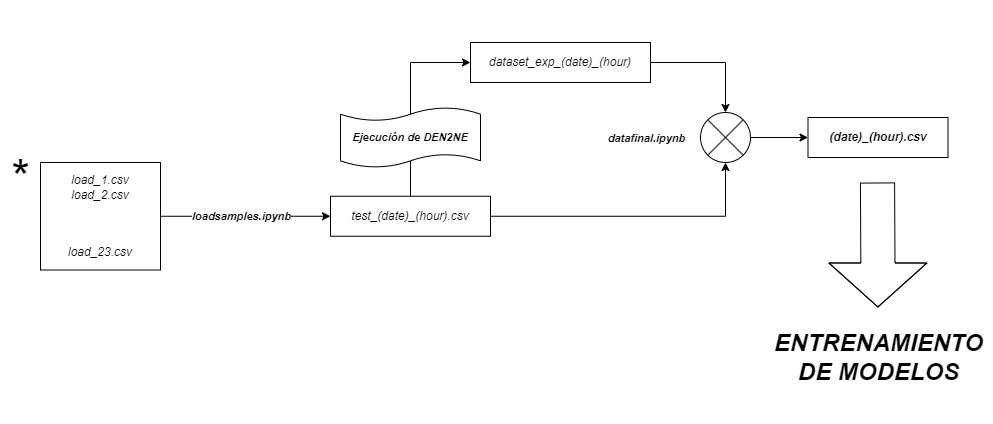
\includegraphics[width=1\textwidth]{img/diseno/total2.png}
    \caption{Diagrama completo de diseño del dataset final}
    \label{fig:total2}
\end{figure}

\vspace{3mm}

Como el objetivo se basa en extraer de los ficheros finales de cargas netas \textit{load\_x.csv} (ver Sección \ref{sec:combinacion}) los datos de los instantes temporales especificados, se introduce un nuevo \textit{notebook}, denominado como \textit{loadsamples.ipynb}. A partir del mismo, se filtran los 12 instantes seleccionados y se obtienen a la salida 12 ficheros de test (ej. \textit{test\_2010-11-28\_11.csv}), los cuales serán proporcionados a la entrada del algoritmo para importar los 23 perfiles reales de carga para cada prueba. Es en este paso cuando se proceden a ejecutar las simulaciones en \gls{den2ne}. La aplicación de cada fichero de test a la entrada proporciona a la salida un nuevo directorio nombrado con el instante temporal que especifica el fichero de test en cuestión (ej. \textit{dataset\_exp\_2010-11-28\_11}). En su interior, se impone una organización de los resultados en 18 carpetas, en función del modelo y del grado de conectividad al que hacen referencia (ej. \textit{barabasi\-200\-6}). Cada una de dichas carpetas consta de 60 ficheros de resultados, que incluyen en su nombre el número de semilla, el criterio del algoritmo, el instante temporal, el grado de conectividad y el modelo (ej. \textit{dataset\_seed\_1\_cr\_0\_t\_2010\-11\-28\_11\_dg\_2\_m\_barabasi.csv}). En la Figura \ref{fig:dirnombres} se expone la nomenclatura especificada para cada uno de los directorios y ficheros de resultados.

\vspace{3mm}

\begin{figure}[h!]
    \centering
    \begin{minipage}{0.4\textwidth}
      \centering
      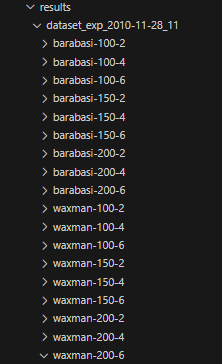
\includegraphics[width=\linewidth]{img/diseno/dirpruebas2.png}
      \label{fig:dirpruebas2}
    \end{minipage}\hfill
    \begin{minipage}{0.6\textwidth}
      \centering
      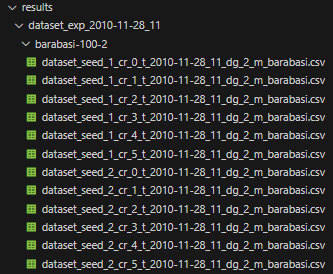
\includegraphics[width=\linewidth]{img/diseno/dirpruebas.png}
      \label{fig:dirpruebas}
    \end{minipage}\hfill
    \caption{Nomenclatura de los directorios y ficheros de resultados}
    \label{fig:dirnombres}
\end{figure}


\vspace{3mm}

Por lo tanto, se puede expresar que para cada prueba ejecutada o fichero de test a la entrada de \gls{den2ne}, se obtienen a la salida un total de 1080 ficheros de resultados. Cada uno de ellos presenta un número de filas igual a la cantidad de nodos de la topología simulada y, en consecuencia, de los intercambios energéticos realizados (100, 150 o 200 filas). 

\vspace{3mm}

Con esto, ya es posible crear el dataset final mediante un nuevo \textit{notebook}, denominado como \textit{datafinal.ipynb}. A modo de simplificar el tratamiento de los resultados del algoritmo, se agrupa primero, en un mismo \textit{dataframe} el contenido de los 1080 ficheros resultantes de cada prueba. Después, se comprueba que el porcentaje total de intercambios erróneos o con exceso de capacidad de enlace no es nulo para la prueba en cuestión. Es decir, si no se obtiene ninguna fila con la etiqueta \textit{link\_overflow} activa, no se podrán predecir errores cuando se desarrollen y se entrenen los modelos y, por ello, se debería utilizar otro instante temporal para las simulaciones.

\vspace{3mm}

Una vez realizada esta comprobación, la siguiente acción se basa en combinar los ficheros de resultados con el resto de medidas que proporcionan los ficheros de test. Las filas de ambos se agrupan a partir del perfil de carga configurado en el nodo origen, especificado por el valor del identificador real. Tras esta operación, el nuevo \textit{dataframe} en \textit{datafinal.ipynb} se constituye por todas las columnas de datos. En este paso es importante revisar y eliminar aquellas que están replicadas, como ocurre en el caso del identificador y la fecha. 

\vspace{3mm}

\begin{lstlisting}[style=Python, caption={Combinación de ficheros de resultados y de test}]
    df_merged = pd.merge(df, df_sim, left_on='origen_id', right_on='iid', how='outer')
\end{lstlisting}

\vspace{3mm}

Finalmente, se almacena el \textit{dataframe} ya limpio en un fichero, cuyo nombre hace referencia al instante temporal de la prueba en cuestión (ej. \textit{2010-12-28\_11.csv}). Este fichero contiene un total de 160920 filas con un valor de etiqueta de error y con toda la información respectiva a cada intercambio energético simulado. Por ello, se define como el conjunto de datos final resultante de una prueba o instante temporal determinado. Como se han ejecutado 12 pruebas, si se agrupan los 12 conjuntos finales, se puede calcular una cantidad total de 1931040 intercambios etiquetados sobre los que entrenar los modelos. De forma adicional, se añade la Tabla \ref{tab:datafinal} para exponer los campos que contienen cada uno de los conjuntos finales.

\vspace{3mm}

\begin{table}[h!]
    \centering
    \begin{tabular}{|c|c|c|}
    \hline
    \rowcolor[HTML]{AAAAAA} 
    \multicolumn{1}{|c|}{\cellcolor[HTML]{AAAAAA}Campo} & \multicolumn{1}{c|}{\cellcolor[HTML]{AAAAAA}Descripción} & Unidades \\ \hline
    \textit{timestamp} & Instante temporal de medida & datetime \\ \hline
    \textit{datetime} & Fecha del valor promedio & datetime \\ \hline
    \textit{H} & Hora del valor promedio & - \\ \hline
    \textit{overflow} & Etiqueta binaria de superación de carga & - \\ \hline
    \textit{cap} & Capacidad del enlace & kW \\ \hline
    \textit{load} & Carga neta (\textit{Dif}) & kW \\ \hline
    \textit{dist} & Distancia & m \\ \hline
    \textit{origen\_id} & Identificador de nodo origen & - \\ \hline
    \textit{dest\_id} & Identificador de nodo destino & - \\ \hline
    \textit{len\_origen\_tag} & Longitud de la etiqueta del nodo origen & - \\ \hline
    \textit{len\_dest\_tag} & Longitud de la etiqueta del nodo destino & - \\ \hline
    \textit{modelo} & Modelo de topología & - \\ \hline
    \textit{criterion} & Criterio de selección de IDs & - \\ \hline
    \textit{degree} & Grado de conectividad & - \\ \hline
    \textit{total\_balance} & Balance de carga global & - \\ \hline
    \textit{abs\_flux} & Flujo total de carga en el nodo raíz & - \\ \hline
    \textit{Diffuse Irradiance} & Índice de radiación difusa (\gls{dif}) & W/m2 \\ \hline
    \textit{Plane of Array Irradiance} & Índice de radiación en el plano del array (\acrshort{poa}) & W/m2 \\ \hline 
    \textit{Ambient Temperature} & Temperatura ambiente & C \\ \hline
    \textit{Cell Temperature} & Temperatura de las células solares & C \\ \hline
    \textit{DC Array Output} & Potencia de salida DC del array & W \\ \hline
    \textit{AC System Output} & Potencia de salida AC del sistema & W \\ \hline
    \textit{Pavg} & Potencia consumida & W \\ \hline
    \textit{Dif} & Carga neta calculada & W \\ \hline
    \end{tabular}  
    \caption{Dataset final obtenido por cada instante temporal probado en \acrshort{den2ne}}
    \label{tab:datafinal}
\end{table}

\vspace{3mm}

Con la obtención de estos 12 ficheros finaliza la etapa de diseño y, por ende, el presente Capítulo. A partir de los resultados obtenidos, se puede expresar de forma concluyente que se cumple el objetivo principal de generar un dataset completo, sobre el cual se entrenarán y desarrollarán los modelos en el Capítulo \ref{cha:desarrollo}. 

